\documentclass[12pt,letter]{article}
\usepackage{mathptmx} % added for time new roman font
\usepackage[left=1in,right=1in,top=1in,bottom=1in]{geometry}
\usepackage[latin1]{inputenc}
\usepackage{amsmath}

% defines all example enviorment
\usepackage[framemethod=tikz]{mdframed} % added for the box around examples
\newtheorem{ex}{Example}
\numberwithin{ex}{section} % allows for the use of example numbers that lign up with the section numbers
\newenvironment{example}{\begin{mdframed}[middlelinewidth=0.5mm]\begin{ex}\normalfont}{\end{ex}\end{mdframed}}

% defines all review enviorment
\usepackage[framemethod=tikz]{mdframed} % added for the box around examples
\newtheorem{re}{Review}
\numberwithin{re}{section} % allows for the use of example numbers that lign up with the section numbers
\newenvironment{review}{\begin{mdframed}[middlelinewidth=2mm,roundcorner=20pt]\begin{re}\normalfont}{\end{re}\end{mdframed}}

% defines all vibration case studies
\newtheorem{vcs}{Vibration Case Studies}
\numberwithin{vcs}{section} % allows for the use of numbers that lign up with the section numbers
\newenvironment{vibration_case_studies}{\begin{mdframed}[linecolor=orange,middlelinewidth=2mm,roundcorner=20pt]\begin{vcs}\normalfont}{\end{vcs}\end{mdframed}}

% defines the quotation enviorment 
\usepackage{xcolor}
\newcommand{\quotebox}[2]{\begin{center}\fcolorbox{white}{blue!15!gray!15}{\begin{minipage}{0.9\linewidth}\vspace{10pt}\center\begin{minipage}{0.8\linewidth}{\space\Huge``}{#1}{\Huge''}{\break\null\hfill} {\small #2}  \end{minipage}\medbreak\end{minipage}}\end{center}}

% defines the definition enviorment 
\newcommand{\definitionbox}[2]{\begin{center}\fcolorbox{white}{blue!15!gray!15}{\begin{minipage}{0.9\linewidth}\vspace{10pt}\center\begin{minipage}{0.8\linewidth} {{\textbf{Definition} - }{#1}: {#2}}\end{minipage}\medbreak\end{minipage}}\end{center}}

\usepackage{amsfonts}
\usepackage{amssymb}
\usepackage{graphicx}
\usepackage{float}
\usepackage{booktabs}
%\usepackage{parskip} % remove all the paragraph indents
\usepackage[textsize=tiny]{todonotes}


\usepackage{setspace}
\usepackage[colorlinks=true]{hyperref}
\usepackage{textcomp} 
\usepackage{multicol} 

% added for MATLAB code
\usepackage[framed]{matlab-prettifier}
\let\ph\mlplaceholder % shorter macro
\lstMakeShortInline"

\lstset{
	style              = Matlab-editor,
	basicstyle         = \mlttfamily,
	escapechar         = ",
	mlshowsectionrules = true,
}



\usepackage{color} % color added for editing
\newcommand{\bl}[1]{\textcolor[rgb]{0.00,0.00,1.00}{#1}}
\newcommand{\gr}[1]{\textcolor[rgb]{0.00,0.50,0.00}{#1}}
\newcommand{\rd}[1]{\textcolor[rgb]{0.75,0.00,0.00}{#1}}
\newcommand{\tl}[1]{\textcolor[rgb]{0,0.6,0.60}{#1}}



%%%%%%%		define the symbols for positive directions		%%%%%%
\makeatletter													%%	
%%					
\newcommand*\curveplus{% positive counterclockwise				%%
	\mathbin{\rotatebox[origin=c]{90}{$\m@th\curvearrowleft$}+}}	%%
%%
\newcommand*\rightplus{% positive right							%%
	\mathpalette\@rightplus\relax}								%%
\newcommand*\@rightplus[1]{%									%%
	\mathbin{\vcenter{\hbox{$\m@th\overset{#1+}{\to}$}}}}			%%
%%	
\newcommand*\upplus{% positive up								%%
	\mathbin{+\mathord\uparrow}}									%%
%%			
\newcommand*\downplus{% positive down							%%		
	\mathbin{+\mathord\downarrow}}								%%
%%		
\newcommand*\downrightplus{% positive down and right			%%	
	\mathbin{+ \rotatebox[origin=c]{-30}{$\m@th\rightarrow$}}}	%%
\makeatother 													%%	
%%%%%%%%%%%%%%%%%%%%%%%%%%%%%%%%%%%%%%%%%%%%%%%%%%%%%%%%%%%%%%%%%%


\usepackage{mathtools}          %loads amsmath as well added for the piece wise function
\DeclarePairedDelimiter\Floor\lfloor\rfloor
\DeclarePairedDelimiter\Ceil\lceil\rceil


\newcounter{NumberInTable}
\newcommand{\LTNUM}{\stepcounter{NumberInTable}{(\theNumberInTable)}}

\newcommand{\Laplace}[1]{\ensuremath{\mathcal{L}{\left[#1\right]}}}
\newcommand{\InvLap}[1]{\ensuremath{\mathcal{L}^{-1}{\left[#1\right]}}}
\renewcommand{\textuparrow}{$\uparrow$}

% Sets the footnotes to be letters, not numbers. This is needed or it's a mix of both. 
\renewcommand*\thefootnote{\alph{footnote}}


\begin{document}
	
	% set the section number, along with figure and equation numbers
	\setcounter{section}{3}	
	\setcounter{figure}{0}   
	\renewcommand\thefigure{\thesection.\arabic{figure}}
	\setcounter{equation}{0}   
	\renewcommand\theequation{\thesection.\arabic{equation}}

	\section{Transfer Function for Vibrating Systems}


		Thus far, this text has only considered forced vibrations for 1-DOF systems excited with forcing functions that can be easily expressed using either sin or cos examples. Therefore, the previously developed solutions are only acceptable for systems with known and simple excitations. This chapter will introduce the concept of transfer functions for solving vibration-related problems. The transfer function, in particular the Laplace transfer function, is an important tool in the study of vibrations as it allows the practitioner to solve for the temporal response of a system for a variety of inputs using a single approach. Examples of force excitation that can be calculated include using this method include:
		\begin{itemize}
			\item sinusoidal
			\item base excitation
			\item impulse
			\item arbitrary input
		\end{itemize}


		\subsection{Transfer Function Method (Generic)}
			Consider the following system

			\begin{figure}[H]
				\centering
				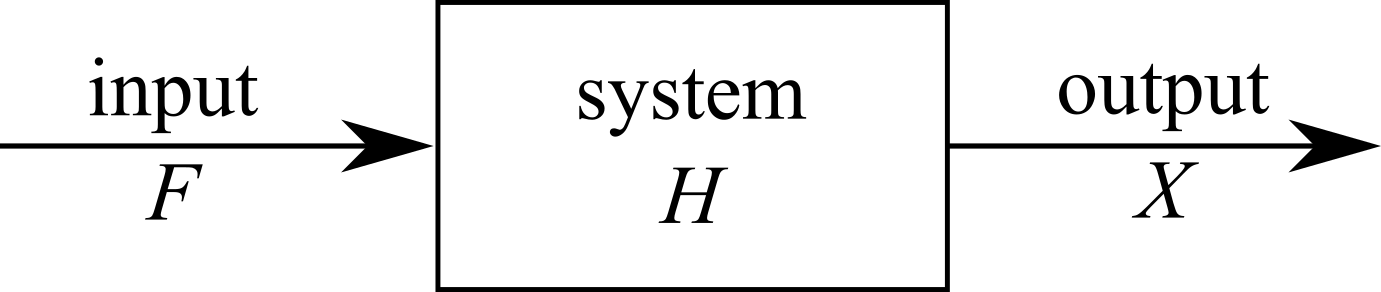
\includegraphics[]{../figures/control_system.png}
				\caption{Generic system $H$ subjected to an input $F$ and its corresponding output $X$.}
				\label{fig:control_system}
			\end{figure}

			\noindent where $F$ is the input, $H$ is the system, and $X$ is the output from the system. This formulation is called the transfer-function approach and is commonly used for the formulation and solution of dynamic problems in the control literature. It can also be used for solving the various forced-vibration problems including those from complex or stochastic inputs. 


\begin{review}
	\label{sec:Laplace_review}
				
		Laplace transforms, or more broadly integral transform, are a procedure for integrating the time ($t$) dependence of a function into a function of position or space ($s$). By transforming the whole differential equation from the time domain into a lower order function of space the problem becomes easier to solve as the function can often be manipulated algebraically. 

		\begin{figure}[H]
			\centering
			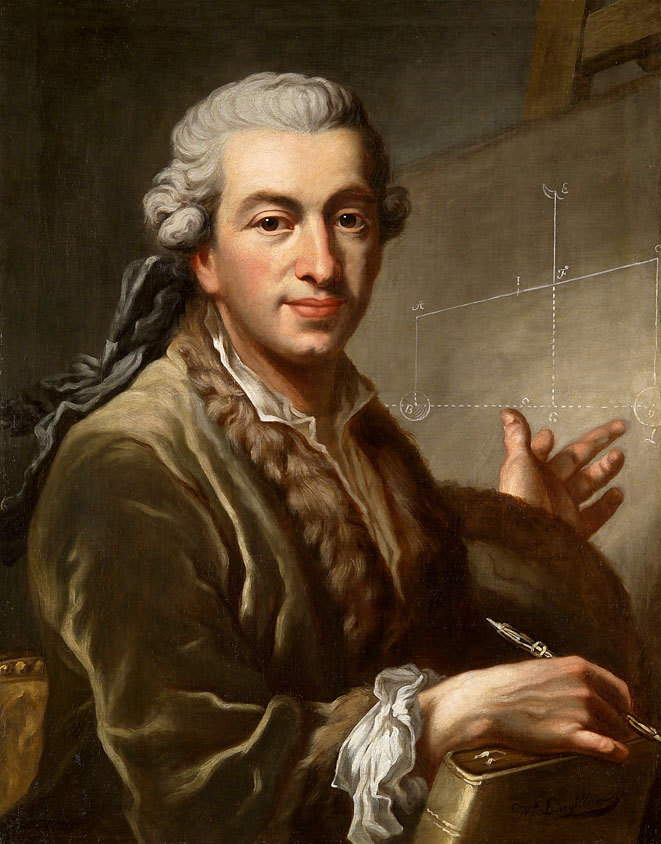
\includegraphics[width=2.71in]{../figures/Pierre-Simon_de_Laplace.jpg}
			\caption{Portrait of Pierre-Simon Laplace by Johann Ernst Heinsius (1775).\protect\footnotemark[1] }
			\label{fig:fragility_curve}
		\end{figure}

		\footnotetext[1]{Johann Ernst Heinsius, CC BY-SA 4.0 $<$https://creativecommons.org/licenses/by-sa/4.0$>$, via Wikimedia Commons}  

		The Laplace transform is named after mathematician and astronomer Pierre-Simon Laplace (23 March 1749 - 5 March 1827 ). Pierre-Simon Laplace was one of the greatest scientists of all time and is often considered the French Newton. He taught Napoleon at the \'Ecole Militaire in 1784, became a count of the empire in 1806, and a marquis in 1817 after the restoration of the monarchy. He is credited with advancements in engineering, mathematics, statistics, physics, astronomy, and philosophy; however, may be his greatest achievement is not only surviving but benefiting from the change from the Ancien R\'egime $\rightarrow$ Bonaparte $\rightarrow$ Bourbon Restoration. 

		
		Of interest to this class is the Laplace transform ($\Laplace{\hspace{1ex}}$) of the function $f(t)$, expressed as $\Laplace{f(t)}$. Here, a Laplace transform is used as a method of solving the differential equations of motion by reducing the computation needed to that of integration and algebraic manipulation. 
		
		The definition of the Laplace transform of the function $f(t)$ is:
		
		\begin{equation}
				\Laplace{f(t)} = F(s) = \int_{0}^{\infty} f(t)e^{-st}dt
		\end{equation}
		where $s$ represents a variable in the complex plane (also called the $s$-plane) and $f(t)=0$ for all values of $t<0$. Here, the $s$ is a complex value. Lastly, the term $F(s)$ is a generic term that  represents the input to a system. As this class needs the derivatives of the base function, we will calculate these next:
		\begin{equation}
			\Laplace{\dot{f}(t)} = \int_{0}^{\infty} \dot{f}(t)e^{-st}dt = \int_{0}^{\infty} e^{-st}\frac{d[f(t)]}{dt}dt 
		\end{equation}		
		integration by parts yields:
		\begin{equation}
			\Laplace{\dot{f}(t)} = e^{-st}f(t)\Big|_0^\infty+s\int_{0}^{\infty}e^{-st}f(t)dt
		\end{equation}
		Astutely, it can be noticed that the second term $s\int_{0}^{\infty}e^{-st}f(t)dt$
		is the input to the system $F(s)$. Therefor, with a little rearranging this becomes:
		\begin{equation}
			\Laplace{\dot{f}(t)} = sF(s)-f(0)
		\end{equation}
		Taking the derivative of again yields:
		\begin{equation}
			\Laplace{\ddot{f}(t)} = s^2F(s)-sf(0)-\dot{f}(0)
		\end{equation}
		
		A few key points of the Laplace transforms are:
				
		\begin{itemize}
			\item The domain of the problem changes from the real number line ($t$) to the complex plane ($s$-plane).
			\item The integration of the Laplace transform changes differentiation into multiplication.
			\item The transform procedure is linear. Therefore, the transform of the linear combination of two transforms is the same as the linear transformation of these functions. 
			\item To move from the time domain to the complex number plane we typically use tables of pre-solved integral. 
			\item The function $x(t)$ can be obtained by taking the inverse Laplace transform defined as $x(t) = \Laplace{X(s)}^{-1}$
		\end{itemize}

			The Laplace transform can be calculated in symbolic form. In particular interest to this text is the Laplace form of the system input $F(s)$ and output $X(s)$. To expand the symbolic form of the Laplace transform for the system inputs are 
			and for system outputs:
			\begin{equation}
				\label{eq:laplace_f}
				\Laplace{f(t)} = F(s)
			\end{equation}		
			\begin{equation}
				\label{eq:laplace_f'}
				\Laplace{\dot{f}(t)} = sF(s)-f(0)
			\end{equation}	
			\begin{equation}
				\label{eq:laplace_f''}
				\Laplace{\ddot{f}(t)} = s^2F(s)-sf(0) - \dot{f}(0)
			\end{equation}	
			here, $f(0)$ and $\dot{f}(0)$ are the initial values of the function $f(t)$.  Furthermore, the for system outputs are:
			\begin{equation}
				\label{eq:laplace_x}
				\Laplace{x(t)} = X(s)
			\end{equation}		
			\begin{equation}
				\label{eq:laplace_x'}
				\Laplace{\dot{x}(t)} = sX(s)-x(0)
			\end{equation}	
			\begin{equation}
				\label{eq:laplace_x''}
				\Laplace{\ddot{x}(t)} = s^2X(s)-sx(0) - \dot{x}(0)
			\end{equation}	
			here, $x(0)$ and $\dot{x}(0)$ are the initial values of the function $x(t)$. 		
	
\end{review}

		\subsection{Transfer Function Method for Solving Vibrating Systems}
		
			As mentioned in the introduction to this chapter, a variety of systems can be solved for using the transfer function method. The procedure for using the Laplace transform to solve equations of motion expressed as an inhomogeneous ordinary differential equation is:
			\begin{enumerate}
				\item Take the Laplace transform of both sides of the EOM while treating the time derivatives symbolically.
				\item Solve for $X(s)$ in the obtained equation.
				\item Apply the inverse transform $x(t) = \Laplace{X(s)}^{-1}$
			\end{enumerate}
				
			\subsubsection{Free Vibration for Undamped Systems}
			Consider the undamped single-DOF system:
			\begin{figure}[H]
				\centering
				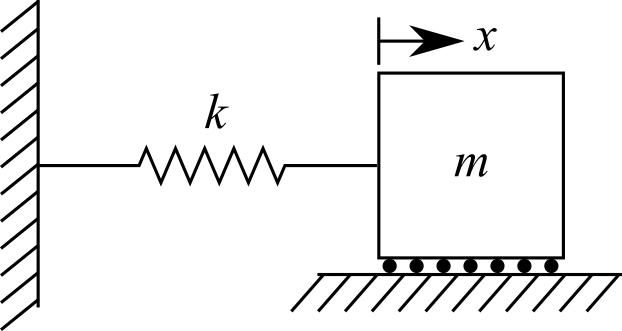
\includegraphics[]{../figures/1-DOF-spring_mass_horizontal.png}
				\caption{A spring mass model of a 1-DOF system.}
			\end{figure}
			\noindent The EOM for this system is a homogeneous differential equation becasue the right-hand side is equal to zero:
			\begin{equation}
				m\ddot{x}(t) + kx(t) = 0 
			\end{equation}
			Here we will leave the ``$(t)$'' for clarity to differentiate the time domain solution from Laplace solution ``$(s)$'' in the $s$-plane, as discussed in review \ref{sec:Laplace_review}. The EOM can be rewritten in standard form as:
			\begin{equation}
				\ddot{x}(t) + \omega_n^2x(t) = 0 
			\end{equation}
			where the initial conditions at $t=0$ are $x(0)=x_0$ and $\dot{x}(0) = v_0$. Taking the Laplace transforms, in symbplic form using equations \ref{eq:laplace_x} - \ref{eq:laplace_x''}, of both sides of the EOM yields:
			\begin{equation}
				\big[s^2X(s) -sx_0 -v_0 \big] + \big[ \omega_n^2X(s) \big] =0
			\end{equation}
			using equations \ref{eq:laplace_x} and \ref{eq:laplace_x''} from section \ref{sec:Laplace_review}. Solving for the output of the system $X(s)$ yields:
			\begin{equation}
			X(s) = \frac{sx_0 + v_0}{s^2 + \omega_n^2}
			\end{equation}
			We can expand this form of $X(s)$ to obtain equations listed in our Laplace Transform table:
			\begin{equation}
			X(s) = \frac{sx_0}{s^2 + \omega_n^2} + \frac{v_0}{s^2 + \omega_n^2}\cdot \frac{\omega_n}{\omega_n}
			\end{equation}
			This becomes:
			\begin{equation}
			X(s) = x_0\frac{s}{s^2 + \omega_n^2} + \bigg(\frac{v_0}{\omega_n}\bigg) \cdot \frac{\omega_n}{s^2 + \omega_n^2}
			\end{equation}
			
			Next, using the inverse Laplace transform $x(t) = \Laplace{X(s)}^{-1}]$ and the two following Laplace transforms (\#5 and \#6):
			\begin{equation}
			f(t) \text{ is cos}(\omega t) \text{ when }  F(s) \text{ is } \frac{s}{s^2+\omega^2} 
			\end{equation}
			\begin{equation}
			f(t) \text{ is sin}(\omega t)  \text{ when }  F(s) \text{ is } \frac{\omega}{s^2+\omega^2} 
			\end{equation}
			Therefore, we can obtain the solution for the system output $X(s)$ as:
			\begin{equation}
			x(t) = x_0 \text{cos}(\omega_n t) + \frac{v_0}{\omega_n}\text{sin}(\omega_n t)
			\end{equation}
			
			The same procedure can be used to calculate the under damped and forced responses. However, when calculating these responses the algebraic solution for $X(s)$, $s$ often contains quotients of polynomials. These Polynomial ratios may not be found in simple Laplace tables and must be solved using the method of partial fractions. An example of this procedure can be found in Appendix B of Inman. 

% this example may not be needed. Check and replace with a better one. 
%			\begin{example}
%				Solve the following system using the transfer function approach:
%				\begin{figure}[H]
%					\centering
%					\includegraphics[width=0.4\textwidth]{../figures/forced_spring_mass_damper_system.png}
%					\caption{Damped 1-DOF spring-mass system subjected to an external force $F(t)$.}
%				\end{figure}
%				\noindent\textbf{Solution:} The system above can be described the the EOM in standard form:
%				\begin{equation}
%				\ddot{x}(t) + 2 \zeta \omega_n \dot{x}+ \omega_n^2x(t) = 0 \text{, where }x(0)=x_0 \text{, and } \dot{x}(0) = v_0 
%				\end{equation}
%				Taking the Laplace transform of both sides of the EOM yields:
%				\begin{equation}
%				\big(s^2X(s) -sx_0 -v_0\big)+\big(s2 \zeta \omega_n X(s)-x_0\big)+\big(\omega_n^2X(s)\big) = 0
%				\end{equation}
%				considering that $sx_0 + x_0$ can be expressed as $sx_0$ because they are both based on the initial condition $x_0$. solving for the output of the system $X(s)$ yields:
%				\begin{equation}
%				X(s) = \frac{sx_0 + v_0}{s^2 + 2 \zeta \omega_n s+ \omega_n^2}
%				\end{equation}
%				Using the method of partial fractions, this can be expressed as inverse Laplace transform $x(t) = \Laplace{X(s)}^{-1}$ resulting in:
%				\begin{equation}
%				F(s) \text{ is } \frac{1}{s^2 + 2 \zeta \omega s+ \omega^2} \text{ when } f(t) \text{ is}\frac{1}{\omega_d}e^{-\zeta \omega t}\text{sin}(\omega_n t),
%				\end{equation}
%				\begin{equation}
%				\text{when } \zeta < 1\text{, and } \omega_d = \sqrt{1-\zeta^2} \nonumber
%				\end{equation}
%				Therefore, we can obtain the solution for the system output $X(s)$ as:
%				\begin{equation}
%				x(t) = x_0 \text{cos}(\omega_n t) + \frac{v_0}{\omega_n}\text{sin}(\omega_n t)
%				\end{equation}
%			\end{example}

\subsubsection{Impulse Response Function}

Shock loads on mechanical systems represent a very common source of vibration. These short-duration forces are also called an impulse. An impulse excitation is defined as a force that is applied for a very short, or infinitesimal, length of time. An impulse is a nonperiodic force that is represented by the symbol $\delta$. The response of a system to an impulse load is the same as the system's free response provided that the correct initial conditions are applied. This is illustrated in the following where the applied force $F(t)$ is impulsive (i.e., large magnitude over a very short time).

\begin{figure}[H]
	\centering
	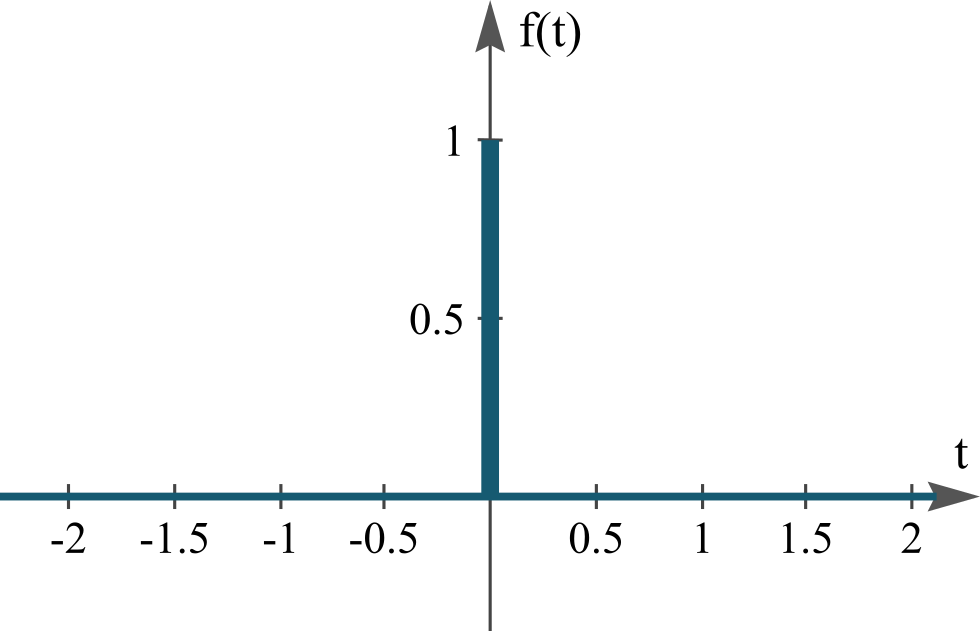
\includegraphics[width=0.5\textwidth]{../figures/unit_impulse.png}
	\caption{An impulse function with the impulse at $t=0$. }
\end{figure}

The impulse response function can be solved for analytically, however, we will solve it using the transfer function approach. Here we will consider the under-damped spring-mass system. First, assume that the system is at rest (no initial conditions). Next, we write the EOM as:
\begin{equation}
m\ddot{x} +c\dot{x} +kx = \delta(t)
\end{equation}
Taking the Laplace transform of both sides of the equation yields 
\begin{equation}
m\big(s^2X(s)-sx(0) - \dot{x}(0)\big) + c\big(sX(s)-x(0)\big) +kX(s) =1
\end{equation}
note that the $\Laplace{\delta}=1$ per \#1 in the transform table. However, if we assume zero initial conditions (a system at rest when the impulse happens), the equation simplifies to. 
\begin{equation}
ms^2X(s) + csX(s) +kX(s) =1
\end{equation}
or
\begin{equation}
(ms^2 + cs +k)X(s) =1
\end{equation}
Solving this equation for $X(s)$:
\begin{equation}
X(s) = \frac{1}{m} \cdot \frac{1}{s^2 + 2 \zeta \omega_n s + \omega_n^2}
\end{equation}
Again, the mass is extracted to develop a formulation that can be found in the Laplace tables. Setting the constraint that $\zeta<1$ and consulting \#10 in the table for Laplace transforms results in:
\begin{equation}
x(t) = \frac{1}{m \omega_d} e^{-\zeta \omega_n t} \text{sin}(\omega_dt)
\label{eq:impulse_load_damped}
\end{equation}
where this is the general solution for a damped system subjected to an impulse loading function. For the undamped case a solution can be obtained by setting $\zeta=0$. This Results in the following form for the undamped case:
\begin{equation}
x(t) = \frac{1}{m \omega_n}\text{sin}(\omega_n t)
\end{equation}
Below is a typical response for both a undamped and underdamped 1-DOF system subject to an impulse response at $t=0$ seconds. 
\begin{figure}[H]
	\centering
	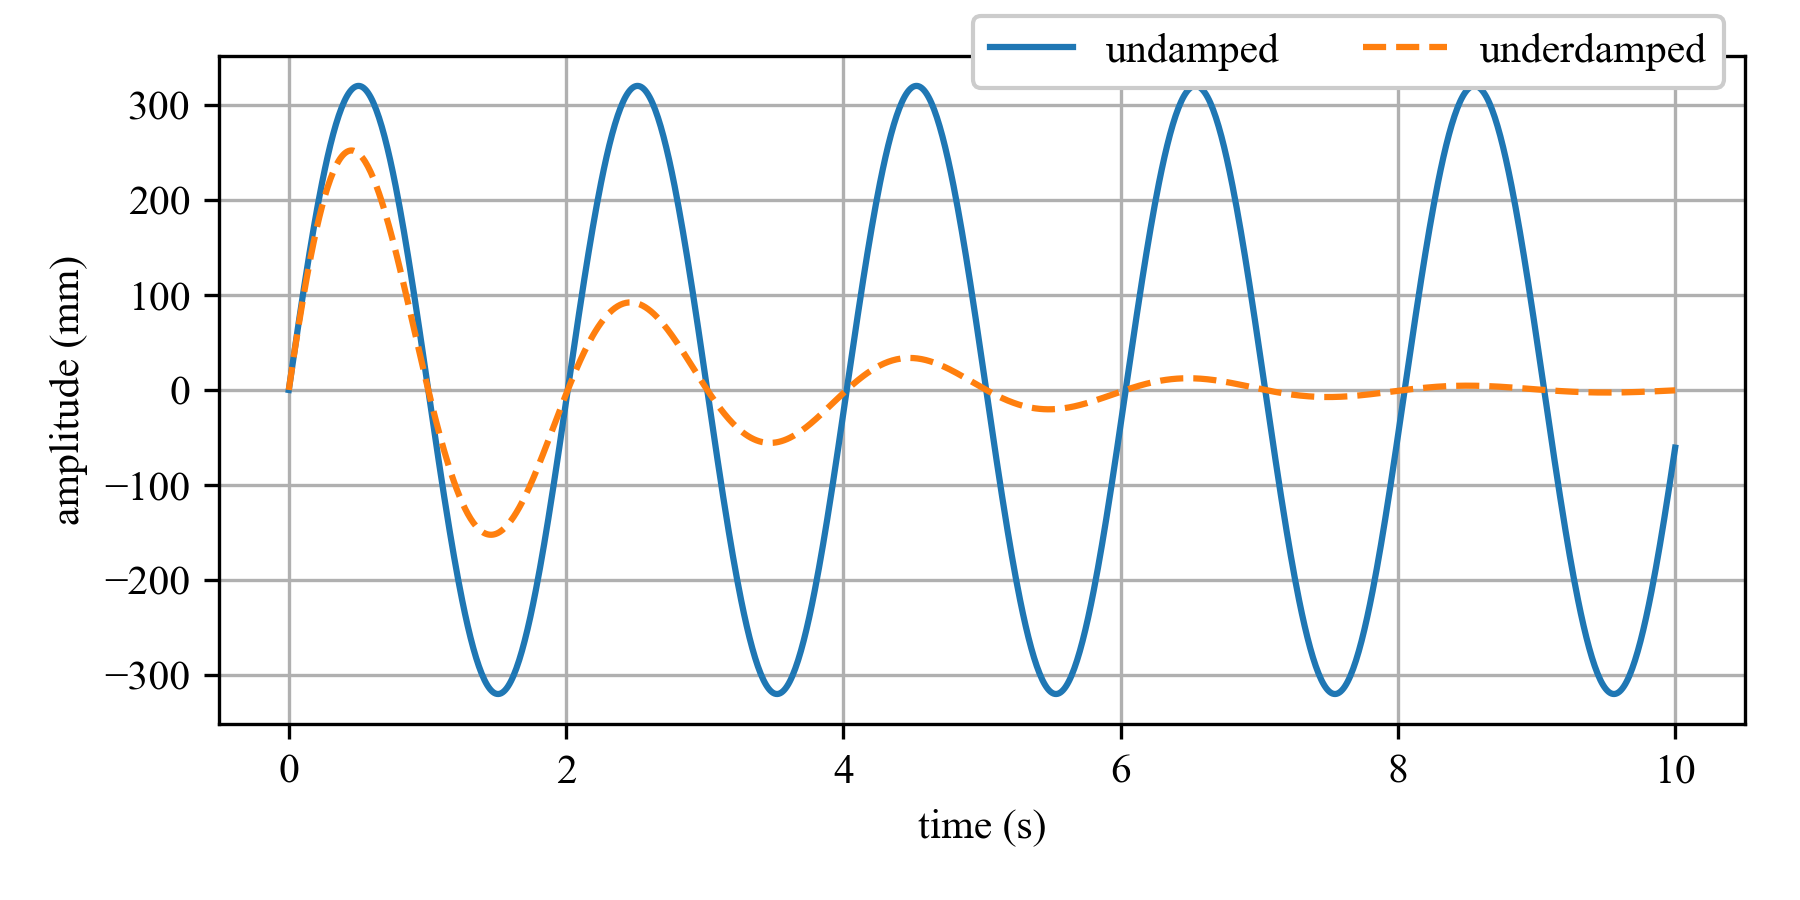
\includegraphics[]{../figures/response_impulse.png}
	\caption{Temporal responses from a underdamped and undamped 1-DOF systems to a impulse response function.}
\end{figure}



\subsubsection{Unit Step function}
Now consider a unit step function, denoted with a capital Greek Phi  $\Phi$: 

\begin{figure}[H]
	\centering
	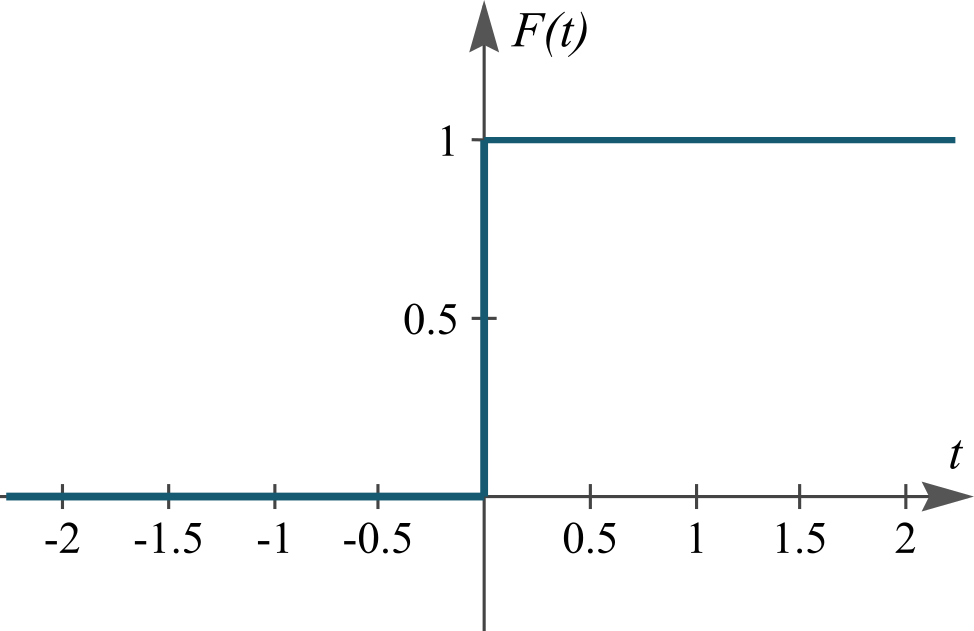
\includegraphics[width=0.5\textwidth]{../figures/unit_step.png}
	\caption{A Step function. }
\end{figure}

A step function is a common loading situation and can represent the dropping of a load into a truck, a car going over a curve, or a motor starting up. 


The Laplace transform of the function, for a unit step function $\Phi$, is: 
\begin{equation*}
\Laplace{\Phi(t)} = \int_{0}^{\infty} e^{-st}dt = -\frac{e^{-\infty}}{s} +\frac{e^{-0}}{s} =\frac{1}{s}
\end{equation*}
This also lines up with Laplace Transform \#3 from the Laplace table. This would be expected as $\Phi$ is used to represent the unit step function (i.e. a step function with a displacement of 1). As we consider linear systems in this class, we can scale the magnitude of the response by the magnitude of the impulse after the transform is performed. 

\subsubsection{Undamped Spring-mass System}

For a spring-mass system subjected to a unit step, assuming both initial conditions are zero, the solution can be obtained using the transform method. First, the EOM is 
\begin{equation}
m\ddot{x}(t) + kx(t) = \Phi(t)
\end{equation}
Taking the Laplace transform of both sides and assuming zero initial conditions yields:
\begin{equation}
	ms^2X(s)+kX(s) =\frac{1}{s}
\end{equation}
Next, this equation is solved for $X(s)$ as:
\begin{equation}
	X(s) = \frac{1}{s(ms^2+k)}
\end{equation}
This can be rearranged as:
\begin{equation}
	X(s) = \frac{1}{m} \cdot \frac{1}{s(s^2+\omega_n^2)}
\end{equation}
where $\frac{1}{m}$ will pass through the Laplace function. Therefore, taking the inverse Laplace transform using \#9 of the provided Laplace transforms yields:
\begin{equation}
	x(t) = \frac{1}{m} \cdot \frac{1}{\omega_n^2}\big(1-\text{cos}(\omega_n t)\big) = \frac{1}{k}\big(1-\text{cos}(\omega_n t)\big)
\end{equation}
 
\subsubsection{Under Damped Spring-mass System}

For a spring-mass-damper system subjected to a unit step, assuming both initial conditions are zero, the solution can be obtained using the transform method. First, the EOM is:
\begin{equation}
m\ddot{x}(t) + c\dot{x}(t) + kx(t) = \Phi(t)
\end{equation}
Converting to the standard form results in:
\begin{equation}
\ddot{x}(t) + 2  \zeta \omega_n\dot{x}(t) + \omega_n^2x(t) = \frac{1}{m} \cdot \Phi(t)
\end{equation}
taking the Laplace transform of both sides and assuming zero initial conditions yields:
\begin{equation}
	s^2X(s) + 2  \zeta \omega_n s X(s) + \omega_n^2 X(s)  =\frac{1}{m} \cdot \frac{1}{s}
\end{equation}
Next, this equation is solved for $X(s)$ as:
\begin{equation}
	X(s) = \frac{1}{s^2 + 2  \zeta \omega_n s + \omega_n^2} \cdot \frac{1}{m} \cdot \frac{1}{s}
\end{equation}
multiplying the right-hand-side of this equation by  $\frac{\omega_n^2}{\omega_n^2}$ results in:
\begin{equation}
	X(s) = \frac{1}{m \omega_n^2} \cdot \frac{\omega_n^2}{s(s^2+2\zeta\omega_n s+\omega_n^2)}
\end{equation}
Again, the $\frac{1}{m\omega_n^2}$ will pass through the Laplace function. Therefore, taking the inverse Laplace transform using \#11 on the Laplace transform sheet yields:
\begin{equation}
	x(t) = \frac{1}{m \omega_n^2} \cdot \Big(1 - \frac{\omega_n}{\omega_d}e^{-\zeta \omega_n t}\text{sin}(\omega_dt + \phi)\Big)\text{, where } \phi = \text{cos}^{-1}(\zeta)\text{, where } \zeta<1
\end{equation}
After obtaining equations for the undamped and under damped cases, the responses for the unit step, solved with the transform method, can be plotted as:
\begin{figure}[H]
	\centering
	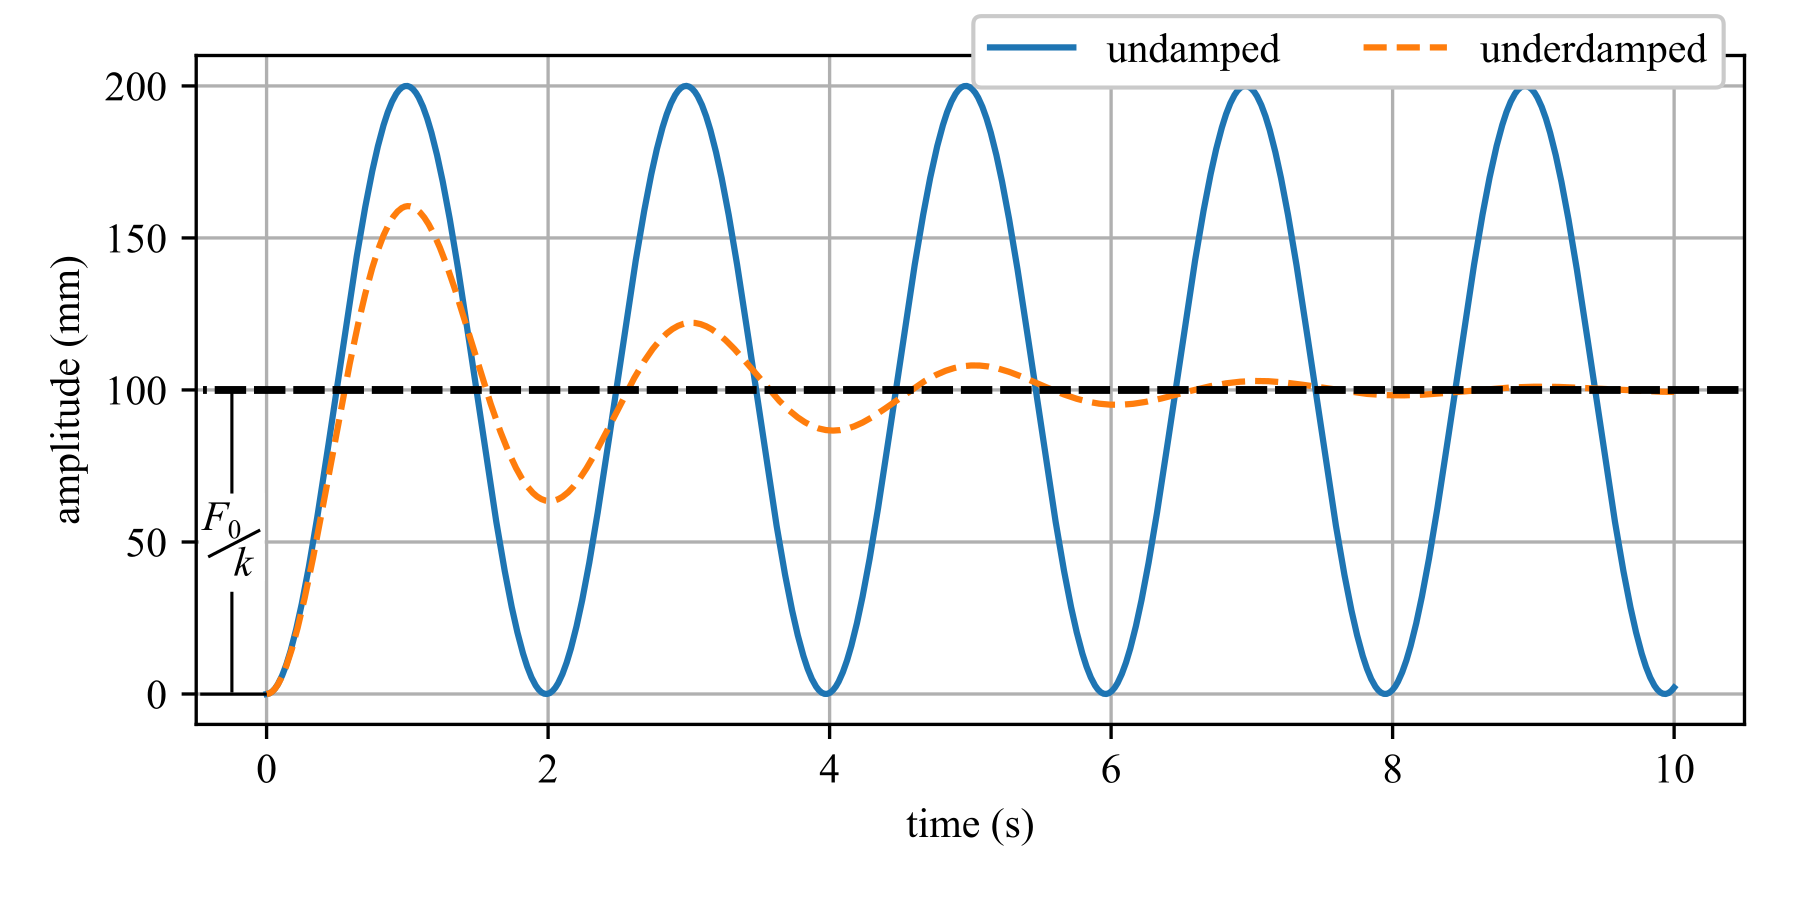
\includegraphics[]{../figures/response_unit_step.png}
	\caption{Temporal responses from underdamped and undamped 1-DOF systems subjected to an impulse response function.}
\end{figure}
Note that the system will settle out around $F_0/k$ where $F_0  \Phi$ is a scaling factor for the step loading.

\begin{example}
A load of dirt $m_r$ is dumped into the back of a dump truck. Assuming the roosters do not move, the bed of the truck can be modeled as a spring-mass-damper system (of values $k$, $m$, and $c$, respectively). Next, the load of roosters is modeled as a force $F(t) = m_r g$ that is applied to the spring-mass-damper system, as illustrated in the following figure. The simplification of the system allows for the analysis of the truck bed's vibrations as a simple spring-mass-damper system. First, assume that the truck's damper is broken, how does the maximum dynamic displacement compare to the static displacement. What would happen to the maximum displacement if the damper was repaired on the truck? %Next, using a damping value of $\zeta=0.5$ and $\omega_n=\pi$ what is the maximum displacement. How does this compare to the displacement for the case without the damper?  

\begin{figure}[H]
	\centering
	\includegraphics[width=0.8\textwidth]{../figures/dump_truck_example.png}
	\caption{Dump truck being loaded with dirt showing (a) dirt going into the truck bed\protect\footnotemark[1]; and (b) the single-degree-of-freedom vibration model.  }
\end{figure}
\footnotetext[1]{SGT Marvin Lynchard, A dump truck is filled with dirt, by members of the 459th Civil Engineering Flight, for use in repairing a damaged runway during Exercise Prime Beef '82, Public Domain, via picryl.com}

\noindent\textbf{Solution:} First, setting the load applied to the truck as 1 unit, it can be seen that this is a unit step loading condition and a broken damper represents an undamped case. To obtain a rough idea about the nature of static and dynamic displacement, the undamped displacement is

\begin{equation}
	x(t) = \frac{1}{k}\big(1-\text{cos}(\omega_n t)\big) = \frac{m_rg}{k}\big(1-\text{cos}(\omega_n t)\big)
\end{equation}
 
This equation has a maximum amplitude when the cos$(\omega_t)=-1$, resulting in:
\begin{equation}
	x(t) = \frac{m_rg}{k}\big(1-(-1)\big)
\end{equation}
This can be rearranged for the maximum displacement value $x_\text{max} $ as:
\begin{equation}
	x_\text{max} = 2\frac{m_rg}{k}
\end{equation} 

Note that the dynamic displacement of the truck bed is twice that of the static displacement. Therefore, if the truck manufacturer designed the truck to only take the static load of rosters (i.e., if the dirt were placed gently into the truck bed), the frame of the truck would be damaged when the dirt were loaded into the truck dynamically. From this, it can be understood that it is important to consider the dynamic responses of a system during the design phase.

%\textbf{Example 1 - under damped}
%For the case where the truck has a damper with a value of $\zeta=0.5$, the displacement $(x)$ can be modeled as:
%\begin{equation}
%	x(t) = \frac{m_rg}{m \omega_n^2} \cdot \Big(1 - \frac{\omega_n}{\omega_d}e^{-\zeta \omega_n t}\text{sin}(\omega_dt + \phi)\Big)\text{, where } \phi = \text{cos}^{-1}(\zeta)
%\end{equation}

\end{example}

\subsection{System Response to Arbitrary Inputs}

\label{sec:impulse_inputs}

The time-domain response of a system to an arbitrary input force in time can be calculated using a series of impulses as shown in figure \ref{fig:Arbitary_excitation_forces}. This method allows the practitioner to easily calculate the response of an arbitrary input to a system using a single expression executed in a ``for loop''. This type of analysis is often more efficient in terms of programing than more direct methods such as the transfer functions shown in this text. 

\begin{figure}[H]
	\centering
	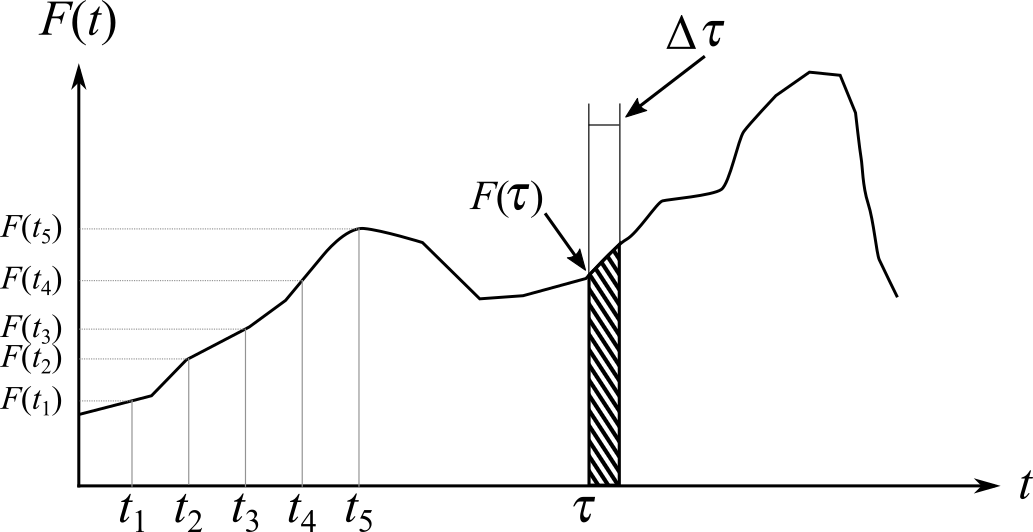
\includegraphics[]{../figures/Arbitary_excitation_forces.png}
	\caption{Generalized response showing that any signal can be represented as a series of impulse signals. }
	\label{fig:Arbitary_excitation_forces}
\end{figure}

To solve for a generalized response to arbitrary inputs, consider that the forces applied in a loop can be expressed as an open-ended summation such that 
\begin{equation}
	\delta x(t) = \sum F( \tau ) g(t- \tau ) \Delta \tau
\end{equation}
By letting $\delta t \rightarrow 0$ the summation can be transferred into the continuous integration  
\begin{equation}
	\delta x(t) = \int_{0}^{t} F( \tau ) g(t- \tau ) d \tau
	\label{eq:Duhamel_1}	
\end{equation}
Knowing the solution to an impulse load, as expressed in equation~\ref{eq:impulse_load_damped}, and inserting this into the prior equation at $g(t)$ we can show that for a system of impulses the total response is
\begin{equation}
	x(t) = \frac{1}{m \omega_d} \int_{0}^{t} F(t) e^{-\zeta \omega_n (t-\tau)} \text{sin}\big(\omega_d(t-\tau)\big) d \tau
	\label{eq:Duhamel_2}	
\end{equation}
Again, this represents the total system response (without initial conditions) for an arbitrary excitation $F(t)$.  These equations are called the \textit{Duhamel} integral. While in many case, the form of function $F(t)$ allows for explicit integration of equations~\ref{eq:Duhamel_1} and \ref{eq:Duhamel_2}. However, numerical evaluation is always possible and many times easier given the simplicity of coding. 



\begin{example}
	
	
	In testing, a hammer is used to excite a 1-DOF system with an impact (i.e. impulse), however, the hammer impacts the system twice by ascendant (a double hit). The first impact has a force of 0.2 N, while the second has a force of 0.1 N and happens 0.1 seconds after the first impact. Plot the response for the double impact. The system has the parameters $m$ = 1 kg, $c$ = 0.5 kg/s, k = 4 N/m. 
	
	\noindent\textbf{Solution:} First, we can define the forcing function as:
	
	\begin{equation}
		F(t) = 0.2 \delta (t) + 0.1 \delta(t-\tau)
	\end{equation}
	where $\tau$ is the offset between the first and second impacts. Next, considering that the unit impulse has a magnitude of 1 we can obtain solutions for the first impact by first writing it's EOM:
	
	\begin{equation}
		m\ddot{x}(t) +c\dot{x}(t) +kx(t) =0.2 \delta(t)
	\end{equation}
	Taking the Laplace transform of both sides of the equation yields 
	\begin{equation}
		m\big(s^2X(s)-sx(0) - \dot{x}(0)\big) + c\big(sX(s)-x(0)\big) +kX(s) = 0.2
	\end{equation}
	However, assuming zero initial conditions, the equation simplifies to. 
	\begin{equation}
		(ms^2 + cs +k)X(s) = 0.2
	\end{equation}
	Solving this equation for $X(s)$:
	\begin{equation}
		X(s) = \frac{0.2}{m} \cdot \frac{1}{s^2 + 2 \zeta \omega_n s + \omega_n^2}
	\end{equation}
	Again, consulting \#10 in the table for Laplace transforms results in:
	\begin{equation}
		x_1(t) = \frac{0.2}{m \omega_d} e^{-\zeta \omega_n t} \text{sin}(\omega_dt)
	\end{equation}
	where this is the general solution for a damped system subjected to an impulse loading function. The second impact can now be solved for using the same method. However, now the time $(t)$ must be offset by $(\tau)$ to allow the impact to still be located at $t=0$ in terms of the second impact. This results in:
	\begin{equation}
		x_1(t) = \frac{0.2}{m \omega_d} e^{-\zeta \omega_n t} \text{sin}(\omega_dt)
	\end{equation}
	\begin{equation}
		x_2(t) = \frac{0.1}{m \omega_d} e^{-\zeta \omega_n (t-\tau)} \text{sin}\big(\omega_d(t-\tau)\big)
	\end{equation}
	Next, using the knowledge that the systems are linear and that the Laplace transform of a linear combination of two transforms is the same as the linear transformation of these functions we can build the piecewise function:
	
	\[
	x(t) = 
	\begin{cases}
		\frac{0.2}{m \omega_d} e^{-\zeta \omega_n t} \text{sin}(\omega_dt) & \text{if } t < \tau \\
		\frac{0.2}{m \omega_d} e^{-\zeta \omega_n t} \text{sin}(\omega_dt)  + \frac{0.1}{m \omega_d} e^{-\zeta \omega_n (t-\tau)} \text{sin}\big(\omega_d(t-\tau)\big) & \text{if } \tau \leq t 
	\end{cases}
	\]
	
	
	For the mass, damping, and stiffness values given above this can be plotted as:
	\begin{figure}[H]
		\centering
		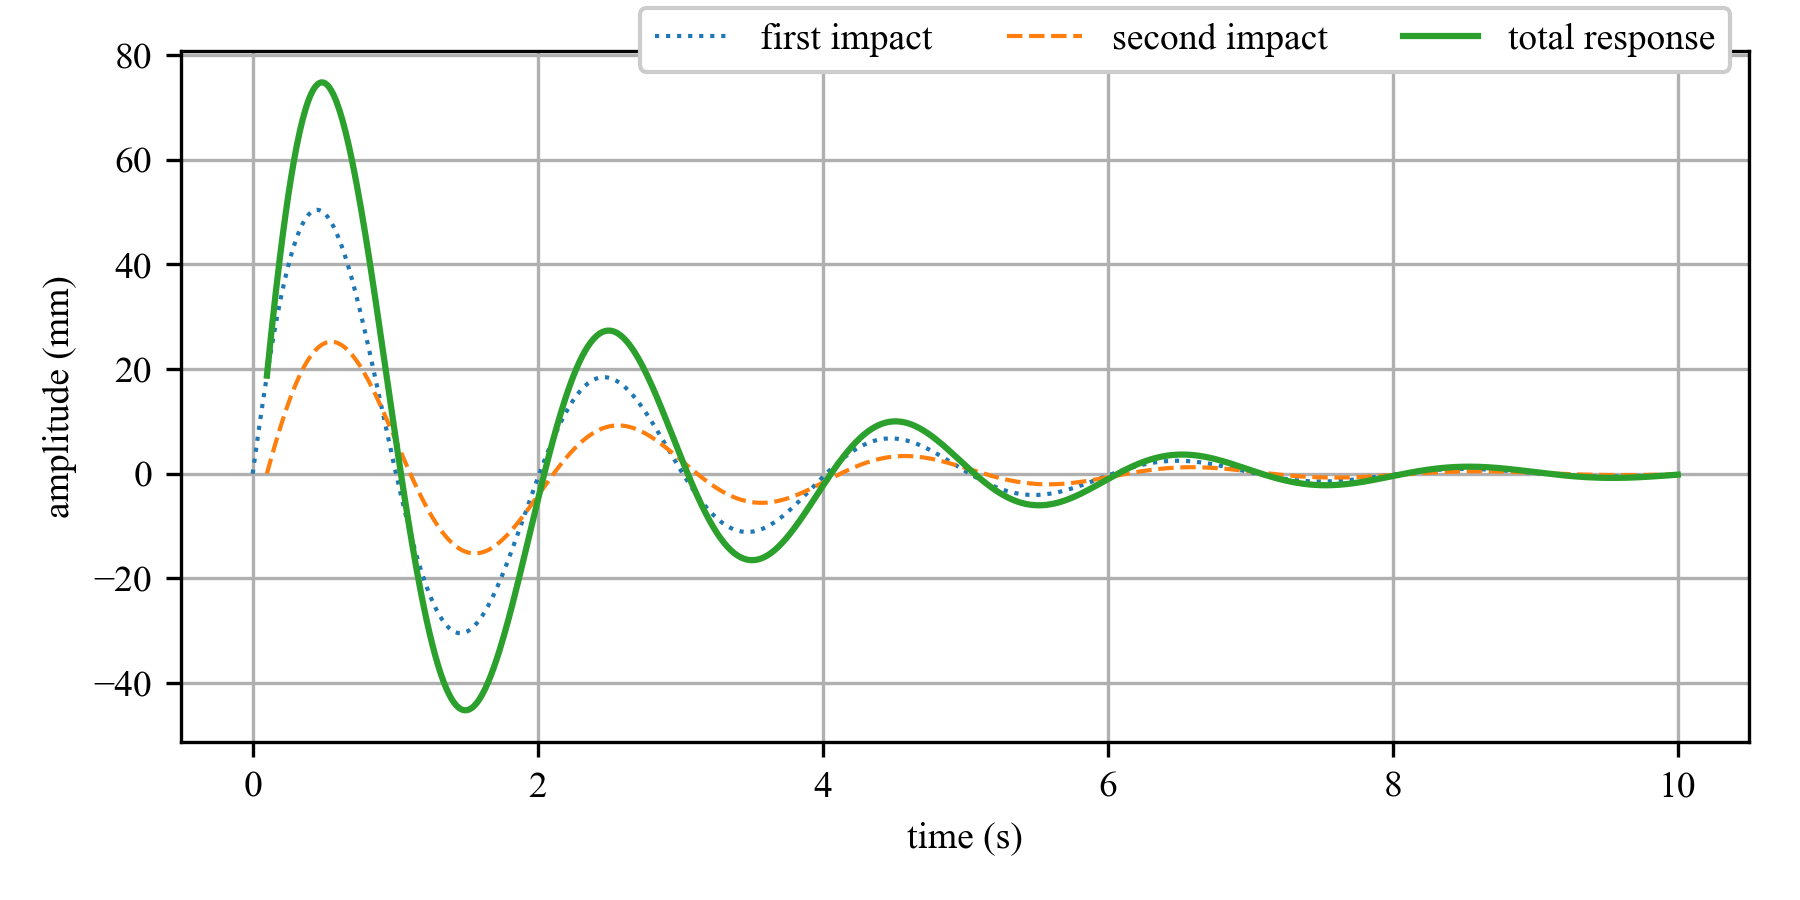
\includegraphics[width=0.75\textwidth]{../figures/response_double_impact.png}
	\end{figure}
	
\end{example}


\begin{example}
	
	Consider the base exciton as shown below subjected to an arbitrary base excitation. Derive an equation (\textit{Duhamel} integral) for its displacement $(z)$, when the displacement is expressed at the relative displacement of the mass such that $z = x - y$. 
	
	\begin{figure}[H]
		\centering
		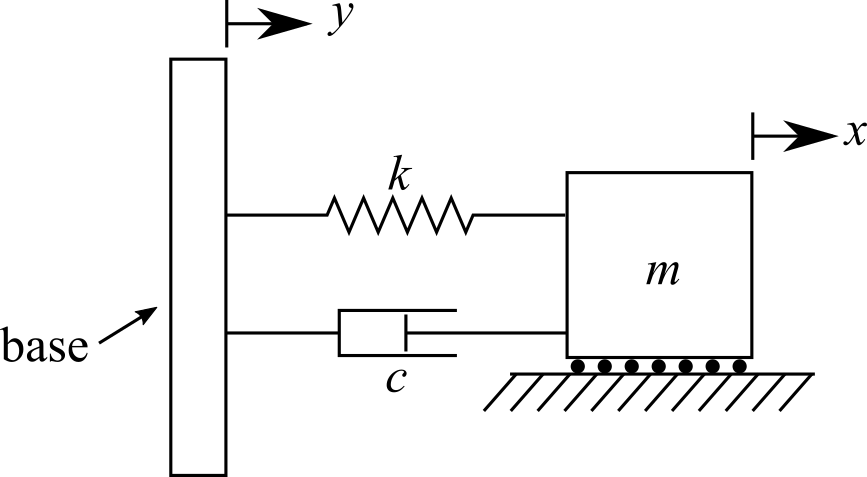
\includegraphics[width=0.35\textwidth]{../figures/1_DOF_spring_dashpot_mass_horizontal_base_excited.png}
		\caption{A base excited 1-DOF spring-mass-damper system.}
	\end{figure}
	
	Defining the EOM for the system results in
	\begin{equation}
		m\ddot{z} + c \dot{z} + kz = -m\ddot{y}
	\end{equation} 	
	Given that we can replace $-m\ddot{y}$ with $F$, this is the same equation as
	\begin{equation}
		m\ddot{z} + c \dot{z} + kz = F
	\end{equation} 	
	meaning that the solutions for an arbitrary force-excited problem can transfer to a base-excited problem if we consider the reletive displacement of the mass. Therefor, we can write the equation for the relative displacement of the mass as
	
	\begin{equation}
		z(t) = -\frac{1}{m \omega_d} \int_{0}^{t} \ddot{y}(t) e^{-\zeta \omega_n (t-\tau)} \text{sin}\big(\omega_d(t-\tau)\big) d \tau	
	\end{equation}
	
\end{example}



\subsection{Transfer Function for Response to Random Inputs}

			Consider the following system
			\begin{figure}[H]
				\centering
				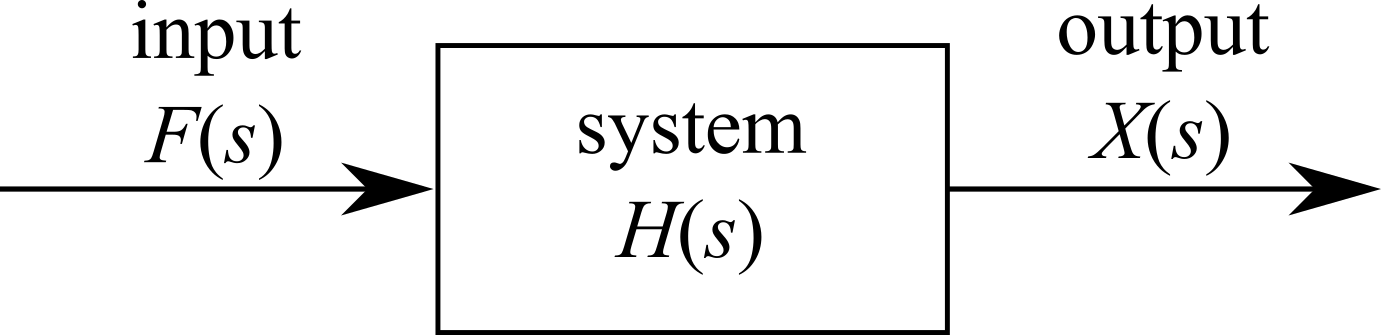
\includegraphics[]{../figures/transfer_function_system.png}
				\caption{Generic block diagram of a system $H(s)$ subjected to an input $F(s)$ and its corresponding output $X(s)$ where the $(s)$ denotes that the considered system is in the $s$-plane.}
				\label{fig:transfer_function_system}
			\end{figure}
			\noindent where $F(s)$ is the input, $H(s)$ is the system, and $X(s)$ is the output from the system. This formulation is called the transfer-function approach and is commonly used for the formulation and solution of dynamic problems in the control literature. It can also be used for solving the various forced-vibration problems including those from complex or stochastic inputs. 
	
\subsubsection{Defining the Transfer Function $\mathbf{H(s)}$}

Again, consider the generic system represented in figure~\ref{fig:transfer_function_system}. For this system representation, $F(s)$ is the Laplace of the transform of the driving force and $H(s)$ is the Laplace transform of the response of the system $h(t)$. 

We need to define transfer function $H(s)$ for a generic system. To do this let us show the reasoning behind the transfer function. Here we will show that the output of any system ($x(t)$) can be related to the input of the system ($f(t)$) through a series of polynomial coefficients ($a$ and $b$). Consider the general $n^{th}$-order linear, time-invariant differential equation that governs the behavior of the dynamic system.

\begin{equation}
a_n\frac{d^nx(t)}{dt^n} + a_{n-1}\frac{d^{n-1}x(t)}{dt^{n-1}} + ... + a_0x(t) = b_m\frac{d^mf(t)}{dt^m} + b_{m-1}\frac{d^{m-1}f(t)}{dt^{m-1}} + ... + b_0f(t)
\end{equation} 
where $x(t)$ is the output and $f(t)$ is the input. Note that this is similar to the formulation we have had before for the EOM. Taking the Laplace transformation of both side of the above equation yields

\begin{eqnarray}
&a_ns^nX(s) + a_{n-1}s^{n-1}X(s) + ... + a_0X(s) + \text{initial condition for } x(t) =   \\
&b_ms^mF(s) + b_{m-1}s^{m-1}F(s) + ... + b_0F(s) + \text{initial condition for } f(t)  \nonumber
\end{eqnarray}
It can be seen that this equation is a purely algebraic expression. If we assume the initial conditions to be zero, the equation reduces to the following:
\begin{eqnarray}
(a_ns^n + a_{n-1}s^{n-1} + ... + a_0)X(s) =  (b_ms^m + b_{m-1}s^{m-1} + ... + b_0)F(s) 
\label{eq:transfer_algebraic_expression}
\end{eqnarray}
if we rearrange equation \ref{eq:transfer_algebraic_expression} to solve for the relationship between the Laplace variables $\big( X(s)$ and $F(s) \big)$ and the algebraic expressions we get:
\begin{equation}
\frac{X(s)}{F(s)} = \frac{b_ms^m + b_{m-1}s^{m-1} + ... + b_0}{a_ns^n + a_{n-1}s^{n-1} + ... + a_0}
\end{equation}
this shows that the ratio of the input algebraic expressions over the output algebraic expressions is equal to the ratio of the output Laplace variable over the input Laplace variable. This shows that we can relate the Laplace variables to the algebraic expressions. Therefore, we can define the transfer function $H(s)$ as: 
\begin{equation}
H(s) = \frac{X(s)}{F(s)}
\label{eq:transfer_function}
\end{equation}
In a more formal term, the transfer function is defined as: ``The ratio of the Laplace transforms of the output or response function to the Laplace transform of the input or forcing function assuming zero initial conditions''.

Equation \ref{eq:transfer_function} can be rearranged to show that the output of the system $X(s)$, can be obtained if we know the input $F(s)$ and the transfer function $H(s)$:
\begin{equation}
X(s) = H(s)F(s)
\end{equation}	


\subsubsection{Transfer Function Method (Steady-state Solution)}

Considering the forced system:
\begin{figure}[H]
	\centering
	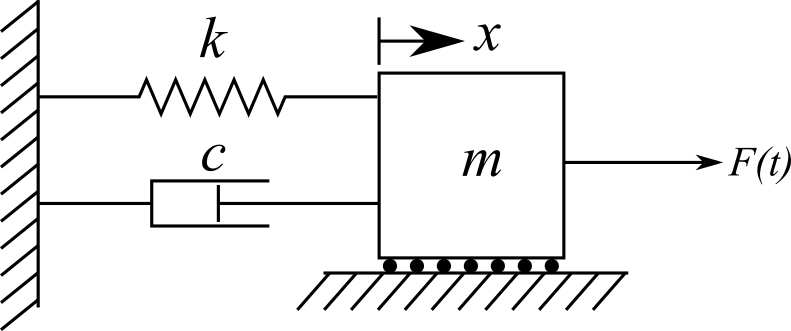
\includegraphics[width=0.4\textwidth]{../figures/1-DOF-spring_dashpot_mass_horizontal_forced.png}
	\caption{A spring-dashpot-mass model of a 1-DOF system with external excitation.}
\end{figure}
\noindent that can be expressed as the equation of motion
\begin{equation}
	m\ddot{x}(t) + c\dot{x}(t) +kx(t) = F_0 \cos(\omega t)
\end{equation}
Here $F_0 \cos(\omega t)$, is used at the input but any input will develope the same transfer function as the transfer function is bounded to the system and not the input. From the \#6 in the table for Laplace Transforms, we know that
\begin{equation}
	\Laplace{\cos(\omega t)} = \frac{s}{s^2+\omega^2}
\end{equation}
Therefore, 
\begin{equation}
F(s) = \frac{F_0s}{s^2+\omega^2}
\end{equation}
Ignoring the initial conditions, and therefore considering only the particular solution, and taking the Laplace transform of the EOM equation yields:
\begin{equation}
(ms^2 + cs +k)X(s) = \frac{F_0s}{s^2+\omega^2} 
\end{equation}
where $X(s)$ denotes the Laplace transform of the unknown function $x(t)$ and $s$ is the complex transform variable. Rearranging the above equation for $X(s)$ yields: 
\begin{equation}
X(s) = \frac{F_0s}{(ms^2 + cs +k)(s^2+\omega^2)}
\end{equation}
Now that we have $F(s)$ and $X(s)$ we can obtain $H(s)$ as  
\begin{equation}
H(s) = \frac{X(s)}{F(s)} = \frac{F_0s}{(ms^2 + cs +k)(s^2+\omega^2)} \cdot \frac{s^2+\omega^2}{F_0s} = \frac{1}{ms^2+cs+k}
\end{equation}
or 
\begin{equation}
H(s) = \frac{1}{ms^2+cs+k}
\end{equation}
This ratio is termed the transfer function of a system and is an important tool in vibration analysis.

Sometimes, how the system responds to an input with certain frequency components is important in understanding the system in general, therefore, we want to solve for the frequency response function of the system. The frequency response function is denoted as $H(j\omega)$ where the complex number $s$ is replaced by the frequency component of the system while considering the imaginary portion in the complex plane (i.e., $s = j\omega$). Therefore, the frequency response function of the system becomes:

\begin{equation}
H(j\omega) = \frac{1}{m(j\omega)^2+cj\omega+k} = \frac{1}{-m\omega^2+cj\omega+k} 
\end{equation}
rearranging into a standard form yields:
\begin{eqnarray}
H(j\omega) = \frac{1}{k-m\omega^2+c\omega j}
\label{eq:frequency_response_function}
\end{eqnarray}
recall that $j^2=-1$. This is the frequency response function of the system. Therefore, it can be seen that the frequency response function of the system is the transfer function of the system evaluated along the imaginary axis $s=j\omega$. However, this expression contains imaginary values (that help to account for the phase in the system) and therefore can be challenging to work with. As the amplitude $|H(j\omega)|$ of the response (the real portion of the equation) is useful to the practitioner, it is prudent to consider the special case of amplitude response while neglecting the phase response. Consider that:
\begin{equation}
	H(j\omega) = \text{R}+\text{I}j
\end{equation}  
so
\begin{equation}
	 |H(j\omega)|=\sqrt{\text{R}^2+\text{I}^2}
\end{equation}  
multiplying $H(j\omega)$ by 1 that is represented by the its unit complex conjugate yields:
\begin{align}
H(j\omega) &= \bigg( \frac{1}{k-m\omega^2+c\omega j} \bigg) \bigg( \frac{k-m\omega^2-c\omega j}{k-m\omega^2-c\omega j}\bigg) \\
&= \bigg( \frac{k-m\omega^2}{(k-m\omega^2)^2(c\omega)^2} \bigg) \bigg( \frac{-c\omega}{(k-m\omega^2)^2(c\omega)^2}j\bigg) 
\end{align}
therefore, $\text{R} = \frac{k-m\omega^2}{(k-m\omega^2)^2(c\omega)^2} $ and $\text{I} = \frac{-c\omega}{(k-m\omega^2)^2(c\omega)^2}$. Now, calculating the amplitude of $H(j\omega)$ we get:
\begin{align}
H(\omega) &= |H(j\omega)| \\
&=  \sqrt{\text{R}^2+\text{I}^2} \\
&=  \sqrt{\frac{(k-m\omega)^2+(-c\omega)^2}{\big((k-m\omega^2)^2+(c\omega)^2)\big)^2}} \\
&=  \sqrt{\frac{1}{(k-m\omega^2)^2+c^2\omega^2}} \\
&= \frac{1}{\sqrt{(k-m\omega^2)^2+c^2\omega^2}}
\end{align}
where $H(\omega)$ represents only the amplitude of the frequency response function and therefore drops the $j$ term from the expression. 


%%%%%%%%%%%%%%%%%%%%%%%%%%%%%%%%%%%%%%%%%%%%%%%%%%%%%%%%%%%%%%%%%%%%%%%%%%%%%%%%%%%%%%%%%%%%%%%%%%%%%%%%%%%%%%%%%%%%%%%%%%%%%%%%%%%%%%%%%
%%%%%%%%%%%%%%%%%%%%%%%%%%%%						Notes on the j therm in H(j\omega)						%%%%%%%%%%%%%%%%%%%%%%%%%%%%

%This as been a point of major debate for myself. My current stance, is Inman drops the j term for convience as he has it with and without in his text, and I can't seem to fully understand why its dropped. 

% Inman 2nd example 5.5.1 has the frequency response function as just $H(\omega)$ I don't know if $H(\omega)$ is standard, as Iman seems to just jump around. }

% Rao 5th in equation 3.55 expresses the "H(i\omega) as the complex frequency response of the system. The absolute value of H(i\omega) given by |H(i\omega)|". As a side note, I like Rao's figure 3.13. That is super cool!

% Rao 5th in section 3.14 Frequency Transfer Functions has information on this

% Rao 5th in section 3.14.2, equaton E.4 says M = |T(i\omega)|. This reincorces the idea that we can define H(\omega) = |H(j\omega)|

%%%%%%%%%%%%%%%%%%%%%%%%%%%%%%%%%%%%%%%%%%%%%%%%%%%%%%%%%%%%%%%%%%%%%%%%%%%%%%%%%%%%%%%%%%%%%%%%%%%%%%%%%%%%%%%%%%%%%%%%%%%%%%%%%%%%%%%%%
%%%%%%%%%%%%%%%%%%%%%%%%%%%%%%%%%%%%%%%%%%%%%%%%%%%%%%%%%%%%%%%%%%%%%%%%%%%%%%%%%%%%%%%%%%%%%%%%%%%%%%%%%%%%%%%%%%%%%%%%%%%%%%%%%%%%%%%%%

\begin{review}
	To recap, for a single DOF damped spring-mass system the transfer function is:
	\begin{equation}
	H(s) = \frac{1}{ms^2+cs+k}
	\end{equation}
	And the frequency response function is: 
	\begin{eqnarray}
	H(j\omega) = \frac{1}{k-m\omega^2+c\omega j}
	\end{eqnarray}
	While the amplitude of the frequency response is:
	\begin{eqnarray}
	H(\omega) = |H(j\omega)| = \frac{1}{\sqrt{(k-m\omega^2)^2+c^2\omega^2}}
	\end{eqnarray}
\end{review}

\begin{example}
	Considering the forced system:
	\begin{figure}[H]
		\centering
		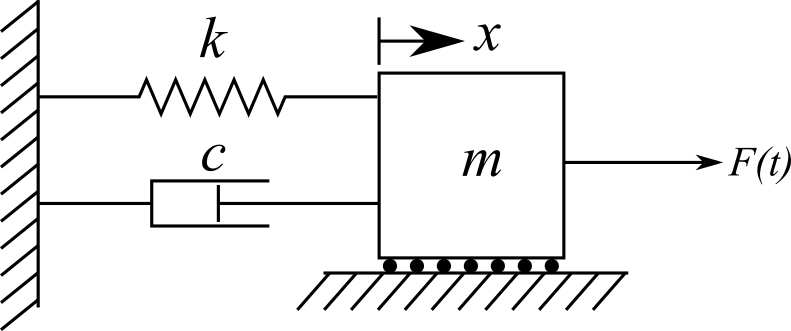
\includegraphics[width=0.4\textwidth]{../figures/1-DOF-spring_dashpot_mass_horizontal_forced.png}
		\caption{A spring-dashpot-mass model of a 1-DOF system with external excitation.}
	\end{figure}
	Set the forcing function to be $F_0 \sin(\omega t)$ and calculate the transfer function. 
	
	\noindent\textbf{Solution:} The equation of motion for the system is:
	\begin{equation}
		m\ddot{x} + c\dot{x} +kx = F_0 \sin(\omega t)
	\end{equation}
	From the \#6 in the table for Laplace Transforms, we know that:
	\begin{equation}
		\Laplace{\sin(\omega t)} = \frac{\omega}{s^2+\omega^2}
	\end{equation}
	Therefore, 
	\begin{equation}
	F(s) = \frac{F_0\omega}{s^2+\omega^2}
	\end{equation}
	Ignoring the initial conditions and taking the Laplace transform of the EOM equation yields:
	\begin{equation}
	(ms^2 + cs +k)X(s) = \frac{F_0 \omega}{s^2+\omega^2} 
	\end{equation}
	Solving algebraically for the $X(s)$ yields: 
	\begin{equation}
	X(s) = \frac{F_0\omega}{(ms^2 + cs +k)(s^2+\omega^2)}
	\end{equation}
	Now that we have $F(s)$ and $X(s)$ we can obtain $H(s)$ as  
	\begin{equation}
	H(s) = \frac{X(s)}{F(s)} = \frac{F_0 \omega }{(ms^2 + cs +k)(s^2+\omega^2)} \cdot \frac{s^2+\omega^2}{F_0 \omega} = \frac{1}{ms^2+cs+k}
	\end{equation}
	or 
	\begin{equation}
	H(s) = \frac{1}{ms^2+cs+k}
	\end{equation}
	This is identical to the solution obtained using $F_0 \cos(\omega t)$ as would be expected because the transfer function is related to the system and not to the input. 
\end{example}  

		\begin{vibration_case_studies}
			Discuss why chimney's are tapered and wind bands. This is useful as wind contains all frequency contents.
			\begin{figure}[H]
				\centering
				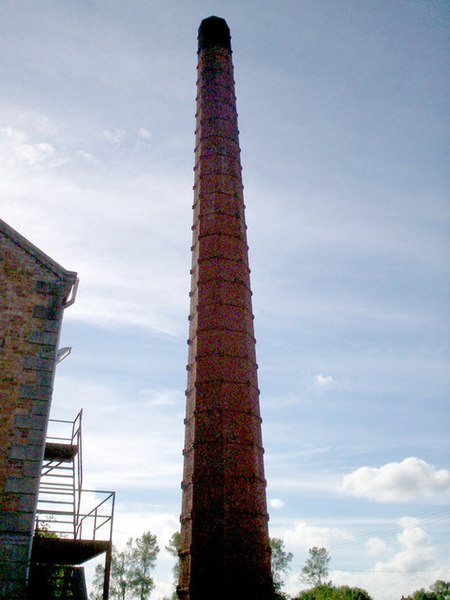
\includegraphics[width=2in]{../figures/tapered_chimney}
				\caption{Tapered chimney with wind bands at a Weaving Factory in the UK \protect\footnotemark[1].}
			\end{figure}
			\footnotetext[1]{P Flannagan / Large Chimney Stack of the disused Weaving Factory, Donaghcloney. / CC BY-SA 2.0} 
		\end{vibration_case_studies}





\subsubsection{Response to Random Inputs}
The transfer and frequency response functions can be very useful for determining the system's response to random inputs. Up to this point, we have solved for deterministic input. 

\begin{itemize}
\item \textbf{Deterministic}-For a known time $t$, the value of the input force $F(t)$ is precisely known. 
\item \textbf{Random} For a known time $t$, the value of the input force $F(t)$ is known only statistically. 
\end{itemize}

To expand, a random signal is a signal with no obvious pattern. For these types of signals, it is not possible to focus on the details of the input signal, as is done with a deterministic signal, rather the signal is classified and manipulated in terms of its statistical properties. 

Randomness in vibration analysis can be thought of as the result of a series of results obtained from testing a system's repeatability for various inputs under varying conditions. In these cases, one record or time history is not enough to describe the system. Rather, an ensemble of various tests are used to describe how the system will respond to the various inputs. 

First, let us consider two inputs, a deterministic input (typical sin wave), and a random input (white noise). These inputs are shown in figure \ref{fig:Response_to_random_input_inputs}. 

\begin{figure}[H]
	\centering
	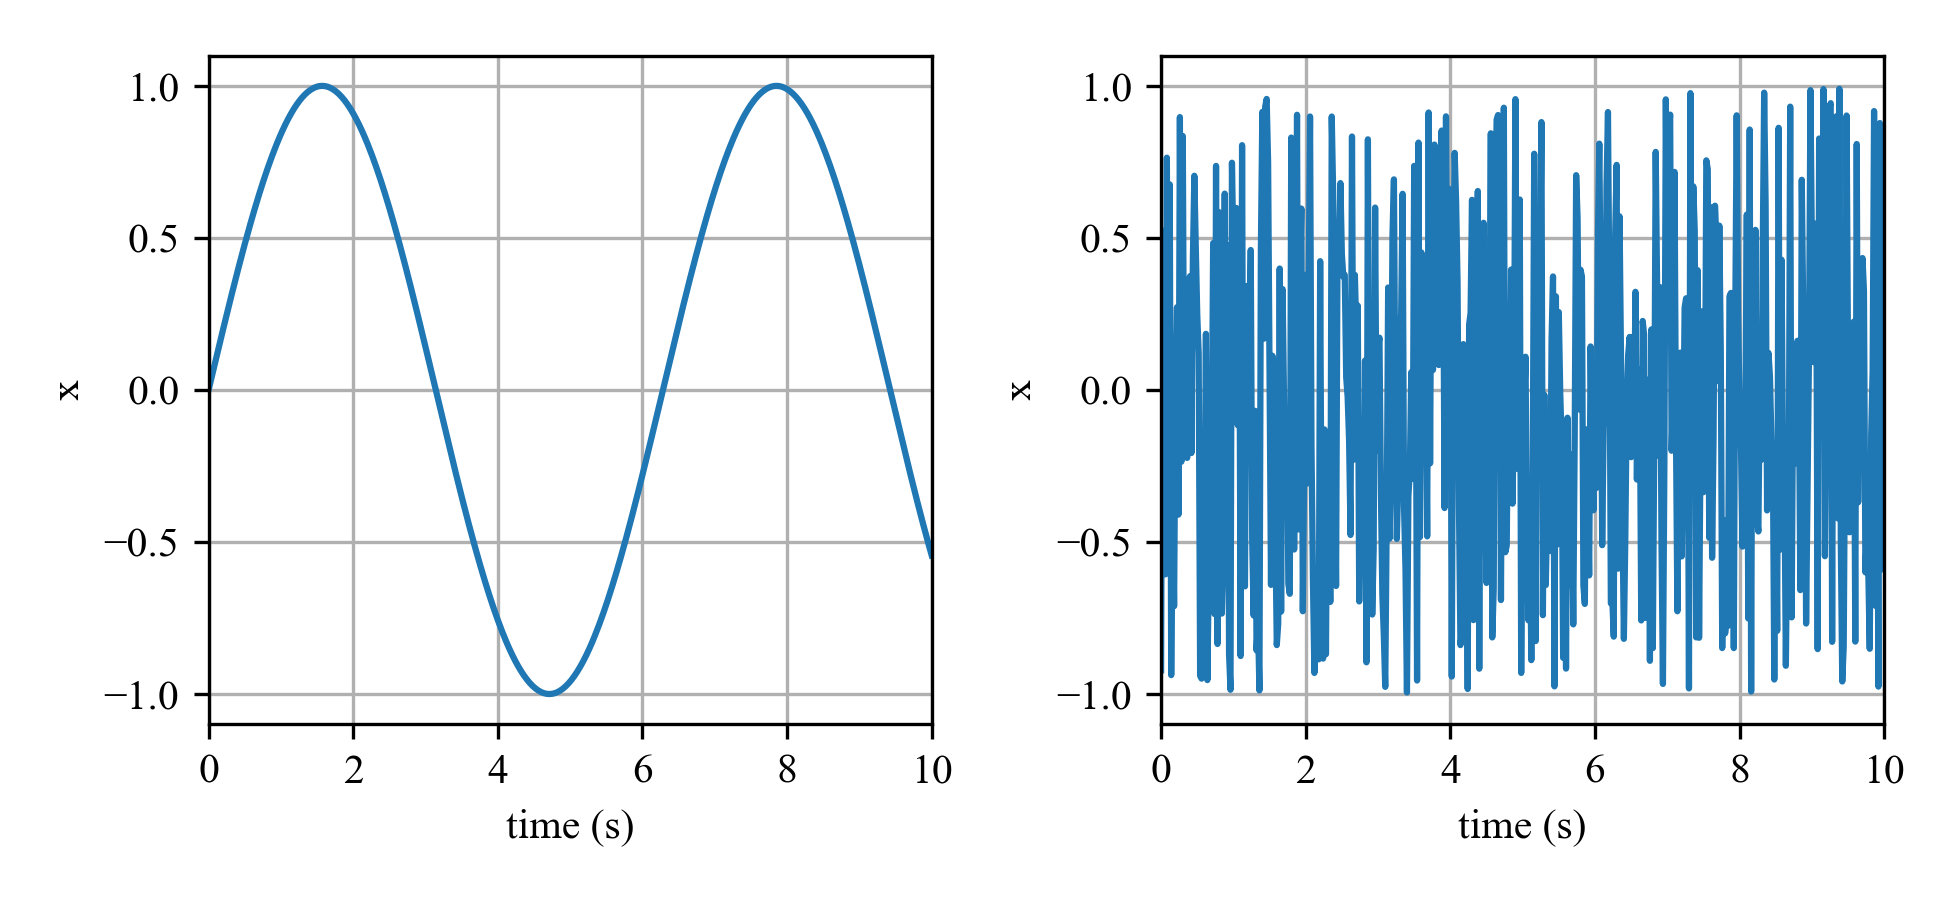
\includegraphics[width=1\textwidth]{../figures/Response_to_random_input_inputs.png}
	\caption{Two arbitrary inputs: (a) sinusoidal; and (b) uniform random noise.}
	\label{fig:Response_to_random_input_inputs}
\end{figure}

One of the first factors to consider is the mean of the random signal $x(t)$, defined as:
\begin{equation}
E[x] = \bar{x} = \lim\limits_{T \rightarrow \infty} \frac{1}{T} \int_{0}^{T}x(t)dt
\end{equation}
where $T$ is the length in time of the data collected. However, for random signals we often want to consider signals with an average mean of zero (i.e. $\bar{x}(t)=0$). Therefore, for signals not centered around zero we can obtain a zero centered signal if the signal is stationary and we subtract the mean value from $\bar{x}$ from the signal $x(t)$. This can be written as:
\begin{equation}
x'(t) = x(t) - \bar{x}
\end{equation} 
where the $x'(t)$ is now centered around zero. As mentioned before, it is important to consider whether or not the input signals are stationary. A signal is stationary if its statistical properties (usually expressed by its mean) do not change with time. Here, it can be seen that for our inputs considered the signals are stationary if a long enough time period is considered. 

Another important variable is variance (or mean-square value) of the random variable $x(t)$ defined as:
\begin{equation}
E[(x-\bar{x})^2] = \lim\limits_{T \rightarrow \infty} \frac{1}{T} \int_{0}^{T}(x(t)-\bar{x})^2dt
\end{equation}
and provides a measure of the magnitude of the fluctuations in the signal $x(t)$. If the signal has an expected value of zero, or $E[x]=0$, this simplifies to. 
\begin{equation}
E[x^2] = \overline{x^2} = \lim\limits_{T \rightarrow \infty} \frac{1}{T} \int_{0}^{T}x^2(t)dt
\end{equation}
This expression leads to the calculation of the root-mean-square (RMS) of the signal:
\begin{equation}
x_\text{rms} = \sqrt{\overline{x^2}} 
\end{equation}

Considering a nonstationary signal, an important measure of interest is how fast the value of the variables changes. This is important to understand as it provides context for how long a signal must be sampled before a meaningful representation of the signal can be calculated in a statistical sense. One way to quantify how fast the values of signal change is the autocorrelation function: 
\begin{equation}
R_{xx}(\tau) = \lim\limits_{T \rightarrow \infty} \frac{1}{T} \int_{0}^{T}x(t)x(t+\tau)dt
\end{equation}
The subscript $xx$ denotes that this is a measure of the response for the variable $xx$, $\tau$ is the time difference between the values at which the signal $x(t)$ is sampled. The auto collation for the two inputs considered above are expressed in figure~\ref{fig:Response_to_random_input_autocorrelation}.
\begin{figure}[H]
	\centering
	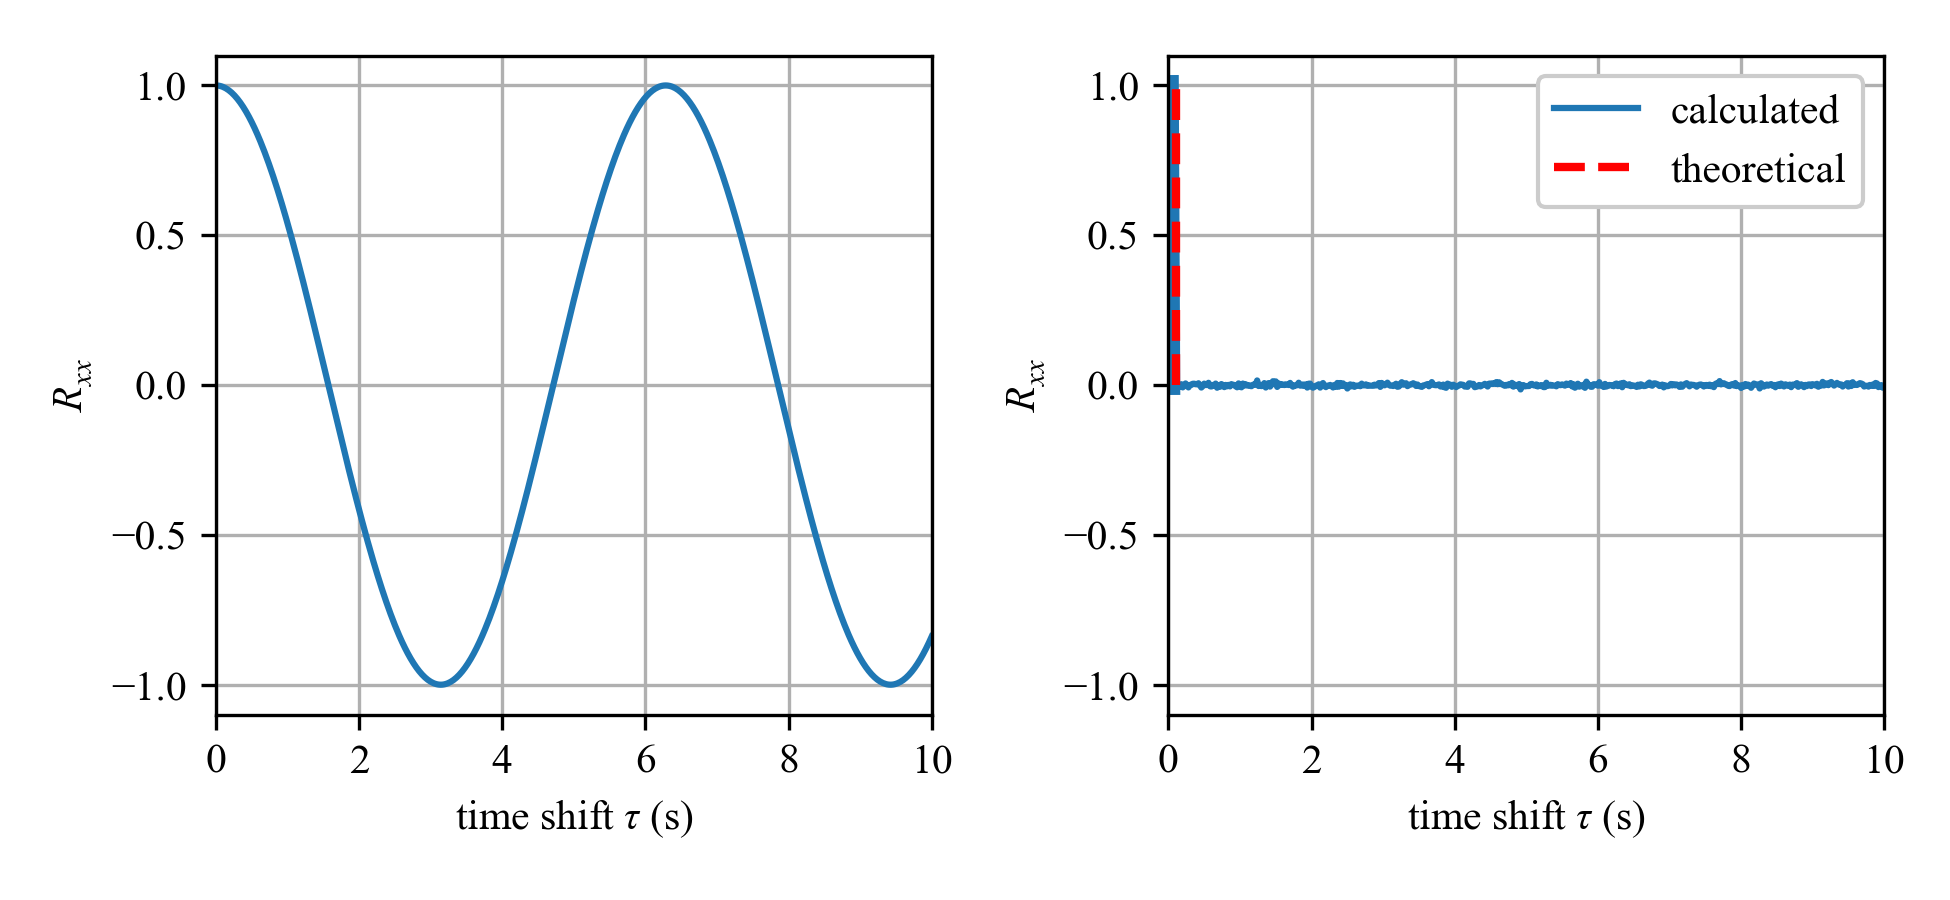
\includegraphics[width=1\textwidth]{../figures/Response_to_random_input_autocorrelation.png}
	\caption{Responses from the autocorrelation function for the inputs shown in figure \ref{fig:Response_to_random_input_inputs} showing: (a) a sinusoidal; and (b) uniform random noise.}
	\label{fig:Response_to_random_input_autocorrelation}
\end{figure} 
\noindent Note that the value of $\tau$ selected in the autocorrelation function greatly affects its response for the sinusoidal input. This is because the values for the sinusoidal are highly correlated. To expand, the value at any time $t$ is greatly effected by the values immediately before and after it. This is not the case for the random input where the signal is not correlated and therefore there is little difference in changing the value of $\tau$ on the response of the autocorrelation function.  

Next, if we take the Fourier transform of the autocorrelation function we obtain the power spectral density (PSD) defined as:
\begin{equation}
S_{xx}(\omega) =\frac{1}{2 \pi} \int_{-\infty}^{\infty} R_{xx}(\tau) e^{-j \omega \tau}d \tau
\end{equation}
where the integral of $R_{xx}(\tau)$ changes the real number $\tau$ into the frequency-domain value $\omega$. The frequency spectrum is denoted with $S$ and the subscript of the considered variable $(\text{e.g., }S_{xx}(\omega))$.  The frequency spectrum for the two input cases considered are plotted in figure~\ref{fig:Response_to_random_input_PSD}.
\begin{figure}[H]
	\centering
	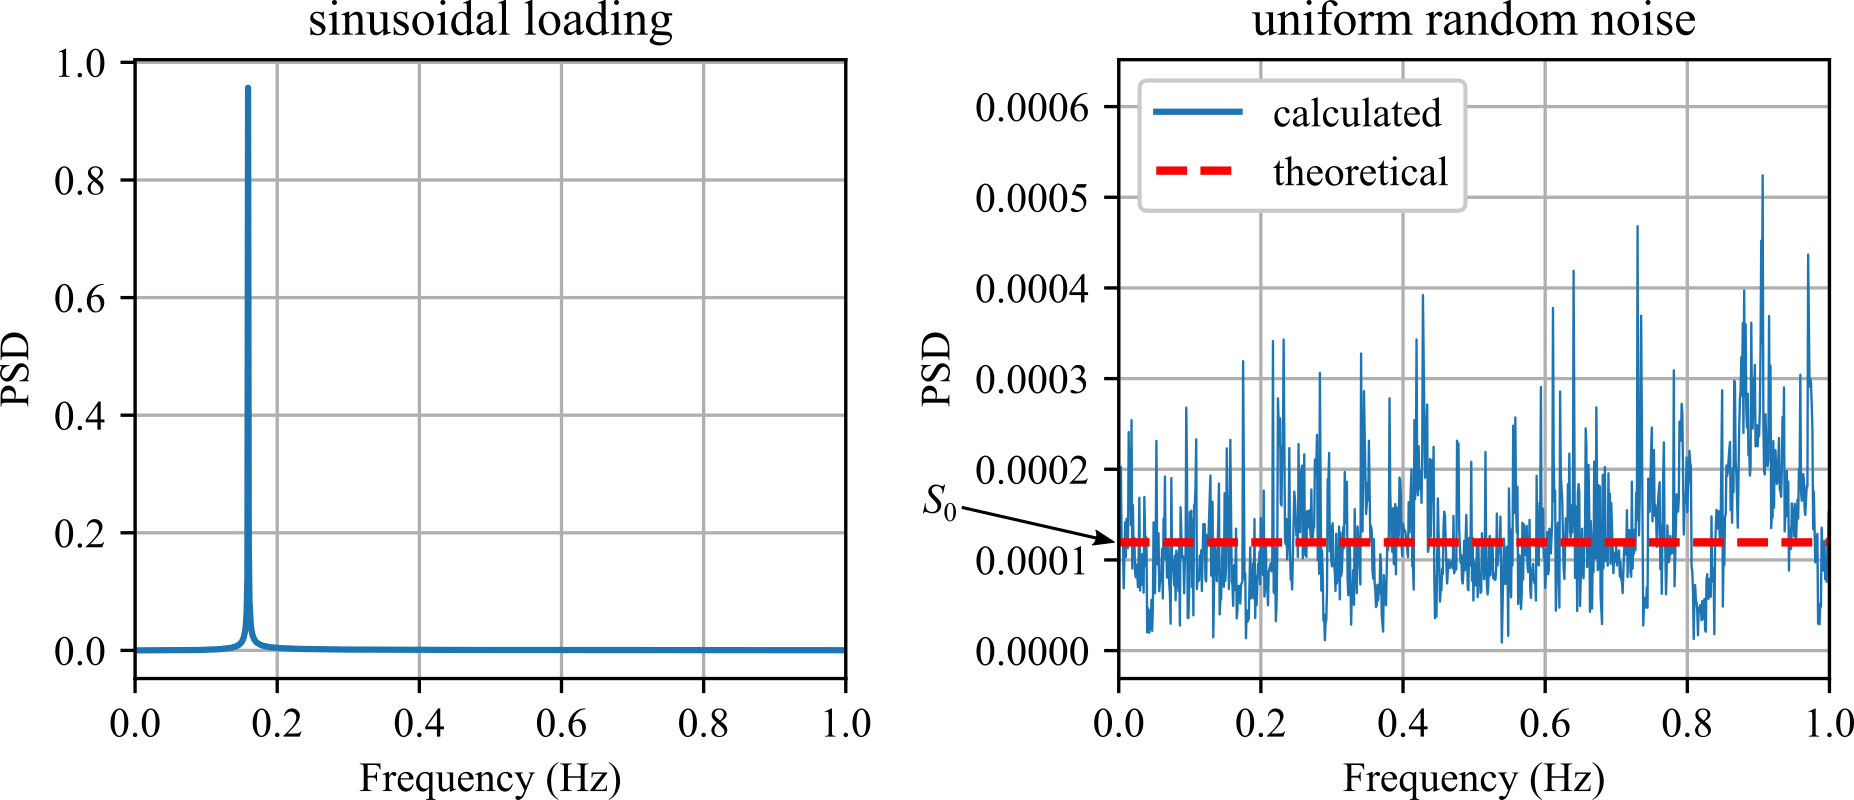
\includegraphics[width=1\textwidth]{../figures/Response_to_random_input_PSD.png}
	\caption{Power spectral density plots for the inputs shown in figure \ref{fig:Response_to_random_input_inputs} showing: (a) a sinusoidal; and (b) uniform random noise.}
	\label{fig:Response_to_random_input_PSD}
\end{figure}
\noindent where the flat frequency response for the random input denotes that the random input is white noise input.  This flat frequency response in the frequency domain can be denoted $S_0$, such that $S_{ff}(\omega) = S_0$ or $S_{xx}(\omega) = S_0$, depending on whether the frequency spectrum of the input $(ff)$ or output  $(xx)$ is being considered. While a true white noise input would be perfectly flat, white noise is really just a theoretical concept as all real-world data will have some variation in the frequency domain as diagrammed in figure \ref{fig:Response_to_random_input_PSD}(b). 

Recall that $S_{xx}$ is the spectrum of the response of the system. For the one-DOF system considered here, we can express the arbitrary input as a series of impulse inputs as discussed in section \ref{sec:impulse_inputs}. This knowledge, along with the frequency response function can be used to relate the spectrum of the input $S_{ff}(\omega)$ to the output through the transfer function as: 

%%%%%%%%%%%%%%%%%%%%%%%%%%%%%%%%%%%%%%%%%%%%%%%%%%%%%%%%%%%%%%%%%%%%%%%%%%%%%%%%%%%%%%%%%%%%%%%%%%%%%%%%%%%%%%%%%%%%%%%%%%%%%%%%%%%%%%%%%
%%%%%%%%%%%%%%%%%%%%%%%%%%%%%%%%%%%%%%%%%%%%%%%%%				Notes			%%%%%%%%%%%%%%%%%%%%%%%%%%%%%%%%%%%%%%%%%%%%%%%%%%%%%%%%%%

% In the equations below, I think my notaion is correct. 

% Inman 2nd edition drops the j, not sure why

% Rao 5th does not drop the i, as shown in equation 10.62. My second equation is the same as Rao's 10.62

%%%%%%%%%%%%%%%%%%%%%%%%%%%%%%%%%%%%%%%%%%%%%%%%%%%%%%%%%%%%%%%%%%%%%%%%%%%%%%%%%%%%%%%%%%%%%%%%%%%%%%%%%%%%%%%%%%%%%%%%%%%%%%%%%%%%%%%%%


\begin{equation}
S_{xx}(\omega) =  |H(j\omega)|^2\Bigg[\frac{1}{2 \pi } \int_{-\infty}^{\infty} R_{ff}(\tau) e^{-j \omega \tau}d  \tau  \Bigg] 
\end{equation}
This can also be expressed in symbolic form as:
\begin{equation}
S_{xx}(\omega) =  |H(j\omega)|^2 S_{ff}(\omega)
\end{equation}
where $R_{ff}$ denotes the autocorrelation function of $F(t)$ and $S_{ff}$ denotes the PSD of the forcing function $F(t)$. The notation $|H(j\omega)|^2$ is the square of the magnitude of the complex frequency response. A more detailed derivation can be found in Rao\protect\footnotemark[1], Inman\protect\footnotemark[2], or Newland\protect\footnotemark[3], but here it is more important to study the results rather than the derivations.

\footnotetext[1]{Singiresu, S. Rao. ``Mechanical vibrations''. Boston, MA: Addison Wesley, 1995.} 
\footnotetext[2]{Inman, Daniel J., and Ramesh Chandra Singh. ``Engineering vibrations''. Vol. 3. Englewood Cliffs, NJ: Prentice Hall, 1994.} 
\footnotetext[3]{Newland, David E. ``Random vibrations, spectral \& wavelet analysis.'' Longman Scientific \& Technical (1993).} 
%\footnotetext[3]{Newland, David E. ``Random vibrations, spectral  wavelet analysis.'' Longman Scientific & Technical (1993).} 

\begin{example}
	Consider the following system
	\begin{figure}[H]
		\centering
		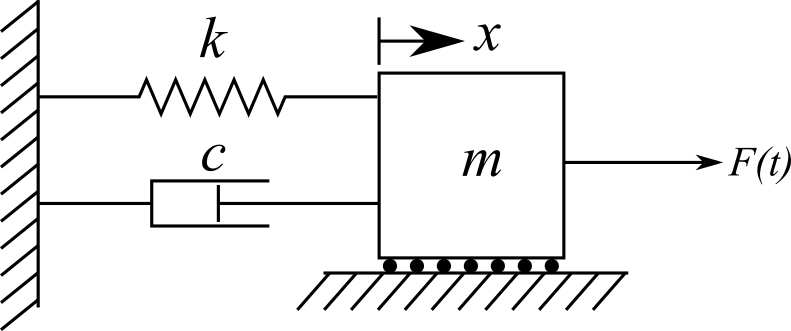
\includegraphics[width=0.4\textwidth]{../figures/1-DOF-spring_dashpot_mass_horizontal_forced.png}
		\caption{A spring-dashpot-mass model of a 1-DOF system with external excitation.}
	\end{figure}
	Calculate the PSD of the response $x(t)$ given that the PSD of the applied force $S_{ff}(\omega)$ is white noise. 
	
	\noindent\textbf{Solution:} From the system we know that the EOM is 
	\begin{equation}
	m\ddot{x}(t) +c\dot{x}(t) + kx(t) = F(t)
	\end{equation} 
	The frequency response function for this system is 
	\begin{eqnarray}
		H(j\omega) = \frac{1}{k-m\omega^2+c\omega j}
	\end{eqnarray}
	while the amplitude of the response is:
	\begin{eqnarray}
	H(\omega) = |H(j\omega)| = \frac{1}{\sqrt{(k-m\omega^2)^2+c^2\omega^2}}
	\end{eqnarray}
	Applying the equation that relates $S_{ff}(\omega)$ to $S_{xx}(\omega)$ we get:
	\begin{equation}
	S_{xx}(\omega) =  |H(j\omega)|^2 S_{ff}(\omega) = \bigg|\frac{1}{k-m\omega^2+c\omega j} \bigg|^2 S_{ff}(\omega) 
	\end{equation}
	White noise means the forcing function $S_{ff}(\omega)$ is constant across the frequency spectrum, therefore, $S_{ff}(\omega)=S_0$. Additionally as:
	\begin{equation}
	|H(j\omega)|^2 = \bigg|\frac{1}{k-m\omega^2+c\omega j} \bigg|^2 = \frac{1}{(k-m\omega^2)^2+c^2\omega^2}
	\end{equation}
	where the absolute value is the amplitude of the system. Therefore, we obtain:
	\begin{equation}
	S_{xx}(\omega) =  |H(j\omega)|^2 S_{0}= \frac{1}{(k-m\omega^2)^2+c^2\omega^2}S_0 = \frac{S_0}{(k-m\omega^2)^2+c^2\omega^2}
	\end{equation}
	Using various values for the elements in the system, the PSD for the system considered looks like:
	\begin{figure}[H]
		\centering
		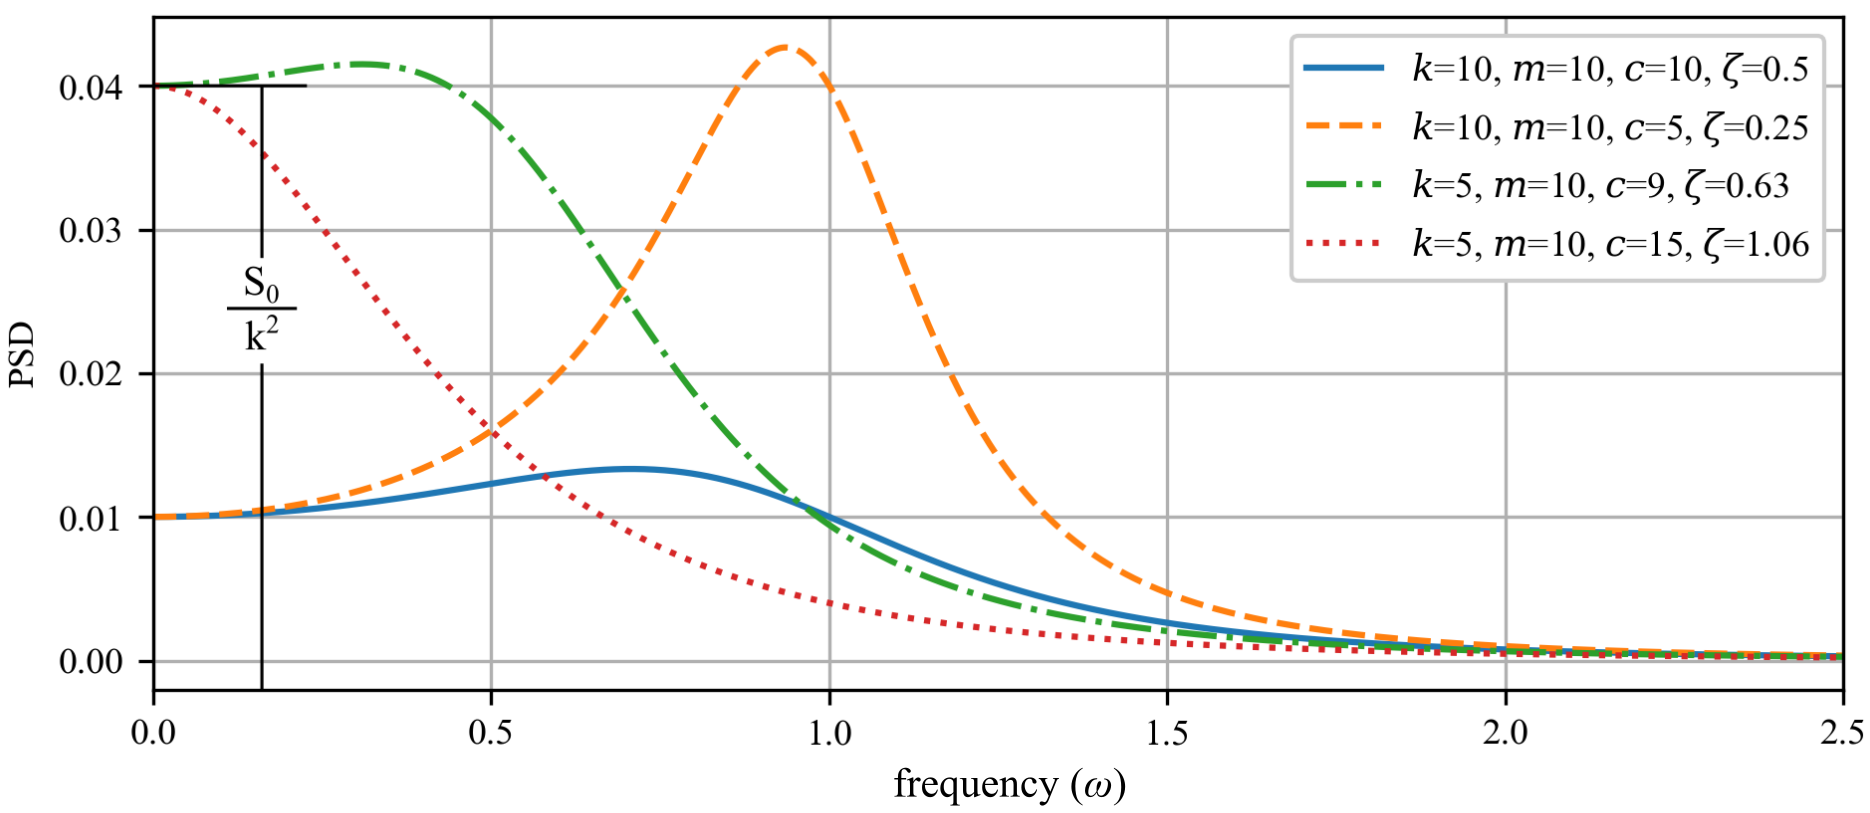
\includegraphics[width=1\textwidth]{../figures/response_to_white_noise_with_annotation.png}
		\caption{Response for considered 1-DOF systems subjected to a white noise input.}
	\end{figure}
\end{example}  

Another useful quantity to consider is the expected output, in terms of its mean and variance, for a given input. Working within the constraint that the system will oscillate about zero, $E[x]=0$, the mean-square value can be directly related to the PSD function as:
\begin{equation}
E[x^2] = \overline{x^2} =   \int_{-\infty}^{\infty} |H(j\omega)|^2 S_{ff}(\omega) d\omega
\end{equation}
For a constant input $S_0$, as diagrammed in figure \ref{fig:Response_to_random_input_PSD}(b), the mean-square value can be expressed as:
\begin{equation}
E[x^2] = \overline{x^2} =   S_{0} \int_{-\infty}^{\infty} |H(j\omega)|^2 d\omega
\label{eq:variance_for_S_O}
\end{equation}

After inspecting the above equation, it becomes clear that to obtain the square of the expected value, a solution for  $\int_{-\infty}^{\infty} |H(j\omega)|^2 d\omega$ must be obtained. For cases where $S_{ff}(\omega) = S_0$ and as such $S_{ff}(\omega)$ can be pulled out of the integral, these integrals have been solved [Random Vibrations, Spectral \& Wavelet Analysis, Newland (1993)]. For example, given $\int_{-\infty}^{\infty} |H(j\omega)|^2 d\omega$:
\begin{equation}
\int_{-\infty}^{\infty} \bigg|\frac{B_0}{A_0+j \omega A_1} \bigg|^2 d\omega = \frac{\pi B_0^2}{A_0 A_1}
\end{equation} 
and
\begin{equation}
\int_{-\infty}^{\infty} \bigg|\frac{B_0 + j \omega B_1}{A_0+j \omega A_1 - \omega^2 A_2} \bigg|^2 d\omega = \frac{\pi (A_0 B_1^2 + A_2 B_0^2)}{A_0 A_1 A_2}
\end{equation} 
When combined with equation \ref{eq:variance_for_S_O}, these integrals allow for the easy calculation of the expected values. 

\begin{example}
	For system below, calculate the mean-square response of the system given that the the spectrum of the input force $F(t)$ is a perfect theoretical white noise.
	\begin{figure}[H]
		\centering
		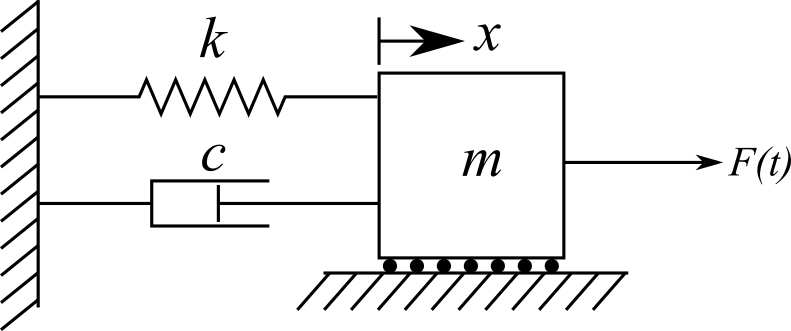
\includegraphics[width=0.4\textwidth]{../figures/1-DOF-spring_dashpot_mass_horizontal_forced.png}
		\caption{A spring-dashpot-mass model of a 1-DOF system with external excitation.}
	\end{figure}
	\noindent\textbf{Solution:} Again, as the forcing function $S_{ff}(\omega)$ is constant across the frequency spectrum $S_{ff}(\omega)=S_0$ the mean-square response can be calculated as:
	\begin{equation}
		E[x^2] = \overline{x^2} =   S_{0} \int_{-\infty}^{\infty} |H(j\omega)|^2 d\omega
	\end{equation}
	Using the already tabulated response:
	\begin{equation}
		\int_{-\infty}^{\infty} \bigg|\frac{B_0 + j \omega B_1}{A_0+j \omega A_1 - \omega^2 A_2} \bigg|^2 d\omega = \frac{\pi (A_0 B_1^2 + A_2 B_0^2)}{A_0 A_1 A_2}
	\end{equation} 
	and the frequency response function for the system as derived in equation \ref{eq:frequency_response_function}:
	\begin{equation}
		H(j\omega) = \frac{1}{k-m\omega^2+c\omega j}
	\end{equation}
	when $B_0=1$, $B_1 = 0$, $A_0=k$, $A_1=c$, and $A_2 =m$. Therefore, using the tabulated expression we can show that:
	\begin{equation}
		E[x^2] = S_0 \frac{\pi m }{k c m} =  \frac{S_0 \pi}{k c}
	\end{equation} 
\end{example}			
			
			
			% Couild add notes on base excitation under random signals. IF so, maybe look at Rao 4.6.1.
			
\pagebreak			
			\pagestyle{empty}
			\newgeometry{top=0.5in, bottom=0.5in,left=0.5in, right=0.5in}
			\vspace{-25ex}
			\begin{center}
			{\large{}\textbf{Table of Laplace Transforms for Vibrations}} \\
			\normalsize{} This is a partial lists of important Laplace transforms for vibrations that assumes \\ zero initial conditions, $0 < t$, and $\zeta < 1$.
			\end{center}
			
			\vspace{0ex}
			{\small
			\renewcommand{\arraystretch}{1.5}
			\begin{multicols}{2}
			\begin{center}
			\begin{tabbing}
			\hspace*{1.5 in}\=\hspace{1.5in}\= \kill
				$f(t)$ \> $\Laplace{f(t)}=F(s)$ \> \\ \noindent\rule{8.0cm}{0.4pt} \\
				$\delta(t)$	\> 1 \> \LTNUM \\ \\
				$\delta(t-t_0)$ \> $e^{-st_0}$ \>\LTNUM \\ \\
				$1$       			 \> $\dfrac{1}{s}$           \>\LTNUM \\ \\
				$e^{at}$ 	\> $\dfrac{1}{s-a}$ 	\>\LTNUM \\ \\
				$\sin (\omega t) $ 	\> $\dfrac{\omega}{s^2+\omega^2}$ \>\LTNUM \\ \\
				$\cos (\omega t) $ 	\> $\dfrac{s}{s^2+\omega^2}$ \>\LTNUM \\ \\
				
				$\sinh (\omega t) $	\> $\dfrac{\omega}{s^2-\omega^2}$ \>\LTNUM \\ \\
				$\cosh (\omega t) $	\> $\dfrac{s}{s^2-\omega^2}$ \>\LTNUM \\ \\
				$\dfrac{1}{\omega^2}\big(1-\cos(\omega t)\big)$ \> $\dfrac{1}{s(s^2+\omega^2)}$ \>\LTNUM \\ \\
				$\dfrac{1}{\omega_d}e^{-\zeta \omega t}\sin(\omega_d t)$ \> $\dfrac{1}{s^2+2\zeta \omega s+\omega^2}$ \>\LTNUM \\ \\
				$1-\dfrac{\omega}{\omega_d}e^{-\zeta \omega t}\sin(\omega_d t + \phi)$, $\phi =\cos^{-1}(\zeta) \dots $ \\ \> $\dfrac{\omega^2}{s(s^2+2\zeta \omega s+\omega^2)}$ \>\LTNUM \\ \\
				$\dfrac{t^{n-1}}{(n-1)!}$, $ n=1,2,\dots $ \> $\dfrac{1}{s^n}$ \>\LTNUM \\ \\
				$t^n $, $n=1,2,\dots$     \> $\dfrac{n!}{s^{n+1}}$    \>\LTNUM \\ \\
				$t^ne^{\omega t}$, $ n=1,2,\dots $	\> $\dfrac{n!}{(s-\omega)^{n+1}}$	\>\LTNUM \\ \\
				$\dfrac{1}{\omega}(1-e^{-\omega t}) $	\> $\dfrac{1}{s(s+\omega)}$	\>\LTNUM \\ \\
				$\dfrac{1}{\omega^2}(e^{-\omega t}+\omega t - 1) $	\> $\dfrac{1}{s^2(s+\omega)}$	\>\LTNUM \\ \\
			\end{tabbing}
			\end{center}
			
			\columnbreak
			
			\begin{center}
			\begin{tabbing}
			\hspace*{1.5in}\=\hspace{1.5in}\= \kill
				$f(t)$ \> $\Laplace{f(t)}=F(s)$ \> \\ \noindent\rule{8.0cm}{0.4pt} \\
				$\dfrac{1}{\omega^3}\big(\omega t - \sin(\omega t)\big) $	\> $\dfrac{1}{s^2(s^2+\omega^2)}$	\>\LTNUM \\ \\
				$\dfrac{1}{2\omega^3}\big(\sin(\omega t) - \omega t \cos(\omega t)\big) \dots $	\\ \> $\dfrac{1}{(s^2+\omega^2)^2}$	\>\LTNUM \\ \\
				$\dfrac{t}{2\omega} \sin(\omega t)$	 \> $\dfrac{s}{(s^2+\omega^2)^2}$	\>\LTNUM \\ \\
				$t\sin (\omega t) $  	\> $\dfrac{2\omega s}{(s^2+\omega^2)^2}$ \>\LTNUM \\ \\
				$t\cos (\omega t) $  	\> $\dfrac{s^2-\omega^2}{(s^2+\omega^2)^2}$ \>\LTNUM \\ \\
				$e^{at}\sin (\omega t) $	\> $\dfrac{\omega}{(s-a)^2+\omega^2}$  \>\LTNUM \\ \\
				$e^{at}\cos (\omega t) $	\> $\dfrac{s-a}{(s-a)^2+\omega^2}$  \>\LTNUM \\ \\
				$e^{at}\sinh (\omega t) $	\> $\dfrac{\omega}{(s-a)^2-\omega^2}$  \>\LTNUM \\ \\
				$e^{at}\cosh (\omega t) $	\> $\dfrac{s-a}{(s-a)^2-\omega^2}$  \>\LTNUM \\ \\
				$\dfrac{1}{\omega_2}\sin(\omega_2 t) - \dfrac{1}{\omega_1}\sin (\omega_1 t) \dots $	 \\ \> $\dfrac{\omega_1^2-\omega_2^2}{(s^2+\omega_1^2)(s^2+\omega_2^2)}$	\>\LTNUM \\ \\
				$\cos(\omega_2 t) - \cos (\omega_1 t)  $	\> $\dfrac{s(\omega_1^2-\omega_2^2)}{(s^2+\omega_1^2)(s^2+\omega_2^2)}$	\>\LTNUM \\ \\
				$e^{at}f(t)$	\> $F(s-a)$	\>\LTNUM \\ \\ 
				$f(t-a)\Phi(t-a)$ \> $e^{-as}F(s)$ \>\LTNUM \\ \\
				$\Phi(t-a)$ \> $\dfrac{e^{-as}}{s}$ \>\LTNUM \\ \\
				$f'(t)$ 	\> $sF(s) - f(0)$ \>\LTNUM \\ \\
			\end{tabbing}
			\end{center}
			\end{multicols}
			}
			
			% Unused Laplace Transforms
			%$f^{n}(t)$ 	\> $s^nF(s) - s^{(n-1)} f(0) - $ \\ \\
			% \> $\cdots - f^{(n-1)}(0)$ \>\LTNUM \\ \\
			%$\displaystyle{\int_0^t f(x)g(t-x)dx}$ \> $F(s)G(s)$ \>\LTNUM \\ \\
			%
			%$t^x$ ($x\geq-1\in\mathbb{R}$)     \> $\dfrac{\Gamma(x+1)}{s^{x+1}}$ \>\LTNUM\\ \\
			%
			%$\dfrac{e^{at}-e^{bt}}{a-b}$	\> $\dfrac{1}{(s-a)(s-b)}$ \>\LTNUM\\ \\ 
			%$f(t)$ \> $\Laplace{f(t)}=F(s)$ \> \\ \\
			%$\dfrac{ae^{at}-be^{bt}}{a-b}$	\> $\dfrac{s}{(s-a)(s-b)}$ \>\LTNUM\\ \\ 
			%$te^{at}$	\> $\dfrac{1}{(s-a)^2}$	\>\LTNUM \\ \\
			%$t\sinh (\omega t) $  	\> $\dfrac{2\omega s}{(s^2-\omega^2)^2}$ \>\LTNUM \\ \\
			%$t\cosh (\omega t) $  	\> $\dfrac{s^2+\omega^2}{(s^2-\omega^2)^2}$ \>\LTNUM \\ \\
			%$\dfrac{\sin (at)}{t}$	\> $\arctan \dfrac{a}{s}$ \>\LTNUM \\ \\
			%$\dfrac{1}{\sqrt{\pi t}}e^{-a^2/4t}$	\> $\dfrac{e^{-a\sqrt{s}}}{\sqrt{s}}$ \> \LTNUM \\ \\
			%$\dfrac{a}{2\sqrt{\pi t^3}}e^{-a^2/4t}$	\> $e^{-a\sqrt{s}}$ \> \LTNUM \\ \\
			%$\text{erfc}\left(\dfrac{a}{2\sqrt{t}}\right)$ \>  $\dfrac{e^{-a\sqrt{s}}}{s}$ \> \LTNUM \\ \\
			% $t^nf(t)$ 	\> $(-1)^n\dfrac{d^nF(s)}{ds^n}$  \>\LTNUM \\ \\
			%{\tiny \textcopyright  2011 B.E.Shapiro for \href{http://integral-table.com}{integral-table.com}. This work is licensed under a} \\
			
			%{\tiny\href{http://creativecommons.org/licenses/by-nc-sa/3.0/}{Creative Commons Attribution-NonCommercial-ShareAlike 3.0 Unported License}. } 
									
\end{document}


























